%=================================================================
% Supplementary Materials -- Control Limits V11
%=================================================================
\documentclass[11pt]{article}

\usepackage[T1]{fontenc}
\usepackage[utf8]{inputenc}
\usepackage{lmodern}
\usepackage[margin=0.95in]{geometry}
\usepackage{microtype}
\usepackage{mathrsfs}
\usepackage{amsmath,amssymb,amsthm,mathtools}
\usepackage{booktabs,array,longtable}
\usepackage{enumitem}
\usepackage[hidelinks]{hyperref}
\usepackage[nameinlink,capitalise]{cleveref}
\usepackage{tikz}
\usetikzlibrary{arrows.meta,positioning,fit,calc,shapes.geometric}
\usepackage{caption}
\usepackage{float}

\setlength{\parskip}{0.42em}
\setlength{\parindent}{0pt}
\setlist{itemsep=0.25em,topsep=0.35em}

%================== macros ==================
\newcommand{\Bbits}{\ensuremath{\{0,1\}}}
\newcommand{\Xspace}{\ensuremath{X}}
\newcommand{\Endo}{\ensuremath{T}}
\newcommand{\Obs}{\ensuremath{O}}
\newcommand{\Tail}{\ensuremath{\Psi}}
\newcommand{\Pred}{\ensuremath{\phi}}
\newcommand{\Diag}{\ensuremath{\mathsf{Diag}}}
\newcommand{\DOne}{\ensuremath{\mathsf{D1}}}
\newcommand{\DTwo}{\ensuremath{\mathsf{D2}}}
\newcommand{\DThree}{\ensuremath{\mathsf{D3}}}
\newcommand{\RCA}{\ensuremath{\mathsf{RCA}_0}}
\newcommand{\ACA}{\ensuremath{\mathsf{ACA}_0}}
\newcommand{\UGapTail}{\ensuremath{\mathsf{UGapTail}}}
\newcommand{\Mspace}{\ensuremath{\mathcal M}}
\newcommand{\ARspace}{\ensuremath{\mathcal A_{R}}}
\newcommand{\Lib}{\ensuremath{\mathcal L}}
\newcommand{\Arch}{\ensuremath{\mathcal A}}
\newcommand{\Inv}{\ensuremath{\mathcal I}}
\newcommand{\FNovel}{\ensuremath{\mathsf{FNovel}}}
\newcommand{\Base}{\ensuremath{\mathfrak B}}
\newcommand{\Task}{\ensuremath{\mathsf Q}}
\newcommand{\im}{\ensuremath{\operatorname{im}}}
\newcommand{\ran}{\ensuremath{\operatorname{ran}}}
\newcommand{\Dec}{\ensuremath{\operatorname{Dec}}}
\newcommand{\Status}{\ensuremath{\mathsf{Status}}}
\newcommand{\N}{\mathbb N}
\newcommand{\R}{\mathbb R}
\newcommand{\Rthree}{\ensuremath{\mathbb R^3}}
\newcommand{\B}{\{0,1\}}
\newcommand{\Pow}{\mathcal P}
\newcommand{\Prf}{\mathsf{Prf}}
\newcommand{\Calc}{\mathsf{Calc}}
\newcommand{\M}{\mathcal M}
\newcommand{\Aud}{\mathsf{Aud}}
\newcommand{\Vis}{\mathsf{Vis}}
\newcommand{\Enc}{\mathsf{Enc}}
\newcommand{\Can}{\mathsf{Can}}
\newcommand{\PCheck}{\mathsf{Check}}
\newcommand{\Novel}{\mathsf{Novel}}
\newcommand{\Sel}{\mathsf{Sel}}
\newcommand{\Img}{\operatorname{Im}}
\newcommand{\rank}{\operatorname{rank}}
\newcommand{\code}{\operatorname{code}}
\newcommand{\sgn}{\operatorname{sgn}}
\newcommand{\quot}{\mathbin{/}}
\newcommand{\eqA}{\mathrel{\sim_{\mathcal A}}}
\newcommand{\qA}{q_{\mathcal A}}
\newcommand{\mc}{\mathcal C}
\newcommand{\mcP}{\mathcal P}
\newcommand{\mcA}{\mathcal A}
\newcommand{\mcH}{\mathcal H_0}
\newcommand{\mcV}{\mathcal V_3}
\newcommand{\Ledger}{\ensuremath{\mathscr L}}
\newcommand{\Debt}{\ensuremath{B}}
\newcommand{\Demand}{\ensuremath{W}}
\newcommand{\AuditCap}{\ensuremath{K}}
\newcommand{\Inflow}{\ensuremath{I}}
\newcommand{\Fin}{\ensuremath{\mathcal P_{\mathrm{fin}}}}
\newcommand{\ViewRec}{\ensuremath{\mathsf{ViewRec}}}
\newcommand{\Coh}{\ensuremath{\mathsf{Coh}}}


\theoremstyle{plain}
\newtheorem{theorem}{Theorem}[section]
\newtheorem{proposition}[theorem]{Proposition}
\newtheorem{lemma}[theorem]{Lemma}
\newtheorem{corollary}[theorem]{Corollary}
\theoremstyle{definition}
\newtheorem{definition}[theorem]{Definition}
\newtheorem{assumption}[theorem]{Assumption}
\newtheorem{hypothesis}[theorem]{Hypothesis}
\newtheorem{construction}[theorem]{Construction}
\newtheorem{example}[theorem]{Example}
\theoremstyle{remark}
\newtheorem{remark}[theorem]{Remark}
\newtheorem{warning}[theorem]{Warning}

\hypersetup{
 pdftitle={Supplementary Materials: Observation Quotients, Orbit Predicates, and the Derivability of Control Limits: Version 11},
 pdfauthor={Andy E. Williams}
}

\title{Supplementary Materials for\\
\large Observation Quotients, Orbit Predicates, and the\\
Derivability of Control Limits\\[2pt]
\large Version 11: Universal M-Space Proof Architecture and Collective Audit Capacity}
\author{Andy E. Williams\\[3pt]
\small Caribbean Center for Collective Intelligence, St.~John's, Antigua and Barbuda\\
\small Nobeah Foundation, Nairobi, Kenya}
\date{2026 -- Version 11}

\begin{document}
\maketitle

\begin{abstract}
This supplement supplies proof expansions, certificate grammars, the exact
coding details for the uniform gap-tail principle, the scoped
functional-novelty ledger, and a full universal M-space proof-architecture
package.  The latter defines communicable proof witnesses, constructs an exact
finite M-space encoding and decoder, proves audit-relative quotient-optimal
compression, constructs audit-preserving three-dimensional visual
realizations, proves their universal graph-theoretic dimension minimality, and
states the exact novelty-separation conditions under which an
audit-equivalent M-space refinement is necessary for reliable derivational
audit.  Version 11 makes the multi-view and capacity conditions explicit:
finite structural audit is relative to a finite admissible projection plan with
finite active support and declared local and global decoders; a single proof
graph is a single-view human audit only when it satisfies the declared
interface bound; and quotient-capacity dominance gives a sufficient
representation-level repair when the quotient itself lies within capacity,
without excluding other repairs that alter a premise of the recurrence.
Application and physical interpretations remain separately bridge-required.
\end{abstract}

\tableofcontents

\section{Status and reading guide}
\label{sec:status}

The main paper has five logically distinct layers:
\begin{enumerate}[label=\textbf{L\arabic*.},leftmargin=2.6em]
\item a quotient/fiber layer;
\item a temporal finite-monitoring versus orbit-target layer;
\item a diagnostic-binding layer;
\item a universal M-space proof-representation and structural-audit layer;
\item a collective proof-audit ledger and capacity layer; and
\item external application, physical, and empirical bridges.
\end{enumerate}

The first four layers supply formal theorems about their declared mathematical
objects.  The ledger layer contains a formal conditional recurrence theorem,
whereas empirical claims about actual repositories and interface performance
remain bridge-required.  The present supplement records the following status
vocabulary:
\[
\{\mathsf{THM},\mathsf{CND},\mathsf{BR},\mathsf{HEUR},\mathsf{OUT},\mathsf{DEF}\}.
\]
Here $\mathsf{THM}$ denotes a proved statement conditional only on its explicit
mathematical hypotheses; $\mathsf{CND}$ a conditional modeling or
representability statement; $\mathsf{BR}$ an application bridge required before
transfer; $\mathsf{HEUR}$ a heuristic; $\mathsf{OUT}$ an excluded conclusion; and
$\mathsf{DEF}$ a stated defeating condition.

\section{Quotient facts and certificate grammar}
\label{sec:quotient}

\begin{definition}[Descent record]
A descent record is a tuple
\[
\mathsf{DescRec}=(X,Z,q,\Psi,\overline\Psi)
\]
with $q:X\to Z$, $\Psi:X\to\Bbits$ and
$\overline\Psi:\im(q)\to\Bbits$ satisfying
\[
\Psi=\overline\Psi\circ q.
\]
\end{definition}

\begin{definition}[Non-descent record]
A paired non-descent record is a tuple
\[
\mathsf{NDescRec}=(X,Z,q,\Psi,x,y)
\]
with
\[
q(x)=q(y),\qquad\Psi(x)\neq\Psi(y).
\]
\end{definition}

\begin{proposition}[Certificate exclusivity]
No pair $(q,\Psi)$ admits both a descent record and a paired non-descent record.
\end{proposition}

\begin{proof}
If a descent record exists, equality $q(x)=q(y)$ gives
$\Psi(x)=\overline\Psi(q(x))=\overline\Psi(q(y))=\Psi(y)$, contrary to the
non-descent condition.
\end{proof}

\begin{proposition}[Quotient criterion, expanded]
\label{prop:fiber-expanded}
Let $q:X\to Z$ and $\Psi:X\to\Bbits$.  The following are equivalent:
\begin{enumerate}[label=\textnormal{(\roman*)},leftmargin=2.6em]
\item there is a decoder $\overline\Psi:\im(q)\to\Bbits$ with
$\Psi=\overline\Psi\circ q$;
\item $\Psi$ is constant on each $q$-fiber;
\item every pair $(x,y)$ with $q(x)=q(y)$ has $\Psi(x)=\Psi(y)$.
\end{enumerate}
\end{proposition}

\begin{proof}
The equivalence of (ii) and (iii) is definitional.  Statement (i) implies (iii)
by substitution.  Under (iii), define $\overline\Psi(z)$ as $\Psi(x)$ for any
$x\in q^{-1}(z)$ when $z\in\im(q)$.  The definition is well formed by (iii), and
then decodes $\Psi$.
\end{proof}

\begin{remark}[Why the image codomain matters]
The decoder is defined only on $\im(q)$.  Nothing in the theorem requires a
choice of values at observations that never occur.  This avoids an unnecessary
surjectivity condition and makes the certificate grammar applicable to arbitrary
channels.
\end{remark}

\section{The rich temporal witness in full detail}
\label{sec:temporal}

\begin{definition}[Propagation and observations]
Let
\[
X=\{A,B\}\times\Bbits^{\mathbb N}\times\mathbb N.
\]
For $x=(\theta,s,i)$, define
\[
T(\theta,s,i)=(\theta,s,i+1),\qquad
 o(\theta,s,i)=s_i,\qquad
 \phi(\theta,s,i)=s_i.
\]
Set
\[
q_n(x)=(o(x),o(Tx),\ldots,o(T^nx)),
\qquad
q_\infty(x)=(o(T^mx))_{m\in\mathbb N}.
\]
\end{definition}

\begin{lemma}[Exact finite monitor decoder]
For every $n\in\mathbb N$, the map
\[
\overline P_n:\Bbits^{n+1}\to\Bbits,
\qquad
\overline P_n(b_0,\ldots,b_n)=1
\Longleftrightarrow b_0=\cdots=b_n=1
\]
satisfies
\[
P_n=\overline P_n\circ q_n,
\]
where $P_n(x)=1$ iff $\phi(T^k x)=1$ for every $k\leq n$.
\end{lemma}

\begin{proof}
For $x=(\theta,s,i)$, the coordinates of $q_n(x)$ are precisely
$(s_i,\ldots,s_{i+n})$.  The condition defining $P_n(x)$ is precisely that all
those coordinates equal $1$.
\end{proof}

\begin{lemma}[Strict refinement]
For every $n$, $q_{n+1}$ is strictly finer than $q_n$.
\end{lemma}

\begin{proof}
The projection deleting the final coordinate maps $q_{n+1}$ to $q_n$, so
$q_{n+1}$ refines $q_n$.  To see strictness, fix $i=0$, take any mode $A$, and
choose streams $s,t$ agreeing at $0,\ldots,n$ but with $s_{n+1}\ne t_{n+1}$.
Then $q_n(A,s,0)=q_n(A,t,0)$ but
$q_{n+1}(A,s,0)\ne q_{n+1}(A,t,0)$.
\end{proof}

\begin{definition}[Latent tail coordinate]
Define
\[
p(A,s,i)=0,\qquad p(B,s,i)=1-\frac{1}{i+1},
\]
and
\[
\Psi(x)=1\quad\Longleftrightarrow\quad
\limsup_{m\to\infty}p(T^m x)<1.
\]
\end{definition}

\begin{lemma}[Mode characterization]
For every $(\theta,s,i)\in X$,
\[
\Psi(\theta,s,i)=1\quad\Longleftrightarrow\quad\theta=A.
\]
\end{lemma}

\begin{proof}
For mode $A$, the sequence $p(T^m x)$ is constantly $0$.  For mode $B$, it is
\[
1-\frac{1}{i+m+1},
\]
which converges to $1$.
\end{proof}

\begin{proposition}[Rich temporal non-descent, expanded]
\label{prop:rich-expanded}
Every $P_n$ descends through $q_n$, the observation tower is strictly refining,
and $\Psi$ does not descend through $q_\infty$.
\end{proposition}

\begin{proof}
The finite part and strictness follow from the preceding lemmas.  Let
$\mathbf 1=(1,1,\ldots)$ and take
\[
x_A=(A,\mathbf 1,0),\qquad x_B=(B,\mathbf 1,0).
\]
Their complete observed streams agree, but the Mode Characterization gives
$\Psi(x_A)=1$ and $\Psi(x_B)=0$.  Proposition~\ref{prop:fiber-expanded} shows
that no decoder through $q_\infty$ exists.
\end{proof}

\begin{lemma}[Shift invariance]
The target $\Psi$ is shift invariant: $\Psi(Tx)=\Psi(x)$ for every $x\in X$.
\end{lemma}

\begin{proof}
Deleting a finite initial segment from a bounded real sequence preserves its
limsup.  The defining condition for $\Psi$ is therefore unchanged by $T$.
\end{proof}

\begin{corollary}[No history-derived repair]
If $r=g\circ q_\infty$ for some $g$, then $\Psi$ does not descend through $r$.
\end{corollary}

\begin{proof}
The pair $(x_A,x_B)$ has equal $q_\infty$ values, hence equal $r$ values, and
unequal $\Psi$ values.
\end{proof}

\begin{definition}[Deterministic finite-state controller]
A deterministic finite-state controller for alphabet $O$ consists of a finite
state set $S$, initial state $s_0$, update $u:S\times O\to S$, and output
$v:S\to\Bbits$.  It reads the orbit observations by
\[
s_{m+1}=u(s_m,o(T^m x)).
\]
It decides $\Psi$ in the eventual-output reading when its output equals
$\Psi(x)$ at all sufficiently late times for every $x$.
\end{definition}

\begin{corollary}[Finite-controller consequence]
No deterministic finite-state controller reading $o$ decides $\Psi$ for the
rich temporal witness in the eventual-output reading.
\end{corollary}

\begin{proof}
The two witness states have the same complete raw input stream, so determinism
forces the same controller trajectory and output sequence on both.  Their
$\Psi$ values differ, hence the common output sequence cannot stabilize correctly
for both.
\end{proof}

\begin{remark}[Separation of resources]
The growing histories $q_n$ and $q_\infty$ are information records, not finite
internal memories.  The finite-controller consequence is supplied separately
because its proof uses bounded state and identical inputs, not merely the
partition theorem.
\end{remark}

\begin{remark}[Interpretive boundary]
This is an existence construction for a declared observation architecture.  It
does not say that all rich histories omit a relevant latent coordinate, nor that
any particular real system contains one.  An external use must supply a bridge
record.
\end{remark}

\section{Wall-refined targets}
\label{sec:wall}

\begin{definition}[Three-valued corridor target]
On
\[
X_\pm=\{A,B_-,B_+\}\times\Bbits^{\mathbb N}\times\mathbb N,
\]
retain the same shift and observed stream and define
\[
W(A,s,i)=\mathsf{safe},\quad
W(B_-,s,i)=\mathsf{left},\quad
W(B_+,s,i)=\mathsf{right}.
\]
The Boolean safety collapse is $\mathrm{Safe}_W=1$ exactly at $\mathsf{safe}$.
\end{definition}

\begin{proposition}[What Boolean safety loses]
The map $r=\mathrm{Safe}_W$ decides $\mathrm{Safe}_W$ but need not distinguish
$\mathsf{left}$ from $\mathsf{right}$.
\end{proposition}

\begin{proof}
Both failure labels map to $0$ under $r$.
\end{proof}

\begin{proposition}[What a wall-valued decoder must retain]
If $W=d\circ r$, then unequal $W$ values imply unequal $r$ values.
\end{proposition}

\begin{proof}
The contrapositive follows by applying $d$ to equal $r$ values.
\end{proof}

\begin{remark}[V5 correction]
A Boolean corridor target does not itself force sign separation.  The separation
claim is sound only after the task codomain is refined to retain the failure-wall
label.
\end{remark}

\section{Diagnostic records and order-two non-factorization}
\label{sec:binding}

\begin{definition}[Diagnostic grammar]
A well-typed record has the form
\[
R=(X,Z,q,\Psi,e,B),
\]
where $q:X\to Z$, $\Psi:X\to\Bbits$, $e$ is either a descent decoder, a paired
non-descent witness, or $\bot$, and $B$ specifies the declared assessment
boundary.  The output is $\DOne$, $\DTwo$, or $\DThree$ respectively.
\end{definition}

\begin{proposition}[Soundness of the status grammar]
For well-typed records:
\[
\DOne\Rightarrow\Dec_q(\Psi),\qquad
\DTwo\Rightarrow\neg\Dec_q(\Psi).
\]
The status $\DThree$ establishes neither conclusion.
\end{proposition}

\begin{proof}
The first implication is the supplied equality $\Psi=\overline\Psi\circ q$.
The second is the supplied fiber violation.  The final claim follows because an
incomplete record is not a proof of a universal negative.
\end{proof}

\begin{definition}[Common library]
Let $\Lib$ denote the class of tuples
\[
L=(X,T,\phi,\Psi,q^0_\infty,q^1_\infty,x_A,x_B,e_0,e_1)
\]
containing both a blind channel $q^0_\infty$ with a valid paired witness $e_0$
and a mode-revealing channel $q^1_\infty$ with a valid decoder $e_1$.
An assembled architecture is
\[
A=(L,\beta),\qquad\beta=(q,\Psi,e,B).
\]
The component projection is $\pi_{\mathrm{cmp}}(A)=L$.
\end{definition}

\begin{construction}[Witness architectures]
For the temporal witness, set
\[
q^0_\infty(\theta,s,i)=(s_i,s_{i+1},\ldots),
\]
\[
q^1_\infty(\theta,s,i)=(\theta,s_i,s_{i+1},\ldots),
\]
\[
e_0=(x_A,x_B),\qquad
 e_1(\theta,t)=\begin{cases}1,&\theta=A,\\0,&\theta=B.\end{cases}
\]
Define
\[
A_0=(L,(q^0_\infty,\Psi,e_0,B)),
\qquad
A_1=(L,(q^1_\infty,\Psi,e_1,B)).
\]
\end{construction}

\begin{lemma}[Output separation]
\label{lem:outputs}
\[
\Diag(A_0)=\DTwo,\qquad\Diag(A_1)=\DOne,
\qquad\pi_{\mathrm{cmp}}(A_0)=\pi_{\mathrm{cmp}}(A_1)=L.
\]
\end{lemma}

\begin{proof}
The first channel has the paired witness $(x_A,x_B)$; the second decoder reads the
mode coordinate.  Both channels and both certificates are retained in the same
library; only the declared binding changes.
\end{proof}

\begin{theorem}[Binding non-factorization]
\label{thm:binding-full}
There is no $d:\Lib\to\{\DOne,\DTwo,\DThree\}$ satisfying
\[
\Diag(A)=d\bigl(\pi_{\mathrm{cmp}}(A)\bigr)
\]
for both $A_0$ and $A_1$.
\end{theorem}

\begin{proof}
A proposed $d$ gives
\[
\DTwo=\Diag(A_0)=d(L)=\Diag(A_1)=\DOne,
\]
contradicting $\DOne\ne\DTwo$.
\end{proof}

\begin{definition}[Scoped functional novelty]
Let $\Base_{\mathrm{cmp}}$ be the class of outputs factoring through
$\pi_{\mathrm{cmp}}$.  The protected invariants are:
\begin{enumerate}[label=\textnormal{(I\arabic*)},leftmargin=2.6em]
\item common-domain typing of each channel and target;
\item attachment of evidence to the channel--target pair it certifies;
\item the stated $\DOne/\DTwo/\DThree$ semantics; and
\item non-promotion of a diagnostic status into an application claim.
\end{enumerate}
\end{definition}

\begin{corollary}[Finite non-substitutability]
The class $\{A_0,A_1\}$ is a finite witness that no member of
$\Base_{\mathrm{cmp}}$ realizes the diagnostic task while retaining the listed
invariants.
\end{corollary}

\begin{proof}
Every member of $\Base_{\mathrm{cmp}}$ has equal output on $A_0$ and $A_1$.
Lemma~\ref{lem:outputs} shows that the correct outputs differ.
\end{proof}

\section{Reverse mathematics: detailed coding proof}
\label{sec:reverse}

\begin{definition}[Uniform gap-tail principle]
For a rational array $a:\mathbb N^2\to\mathbb Q\cap[0,1]$, let
\[
\mathrm{Below}(a,e)\iff
\exists k\exists M\forall m\geq M\;a(e,m)\leq1-2^{-k},
\]
\[
\mathrm{AtOne}(a,e)\iff
\forall k\forall M\exists m\geq M\;a(e,m)>1-2^{-k}.
\]
The gap promise is $\mathrm{Gap}(a,e)\iff\mathrm{Below}(a,e)\vee
\mathrm{AtOne}(a,e)$.  The principle $\UGapTail$ is
\[
\forall a\left[
\forall e\;\mathrm{Gap}(a,e)
\rightarrow
\exists Y\;\forall e\bigl(e\in Y\leftrightarrow\mathrm{Below}(a,e)\bigr)
\right].
\]
\end{definition}

\begin{theorem}[Formal reverse-mathematical equivalence]
Over $\RCA$,
\[
\UGapTail\leftrightarrow\ACA.
\]
\end{theorem}

\begin{proof}
\medskip\noindent\textbf{\(\ACA\Rightarrow\UGapTail\).}
For fixed $a$, the matrix
\[
\exists k\exists M\forall m\geq M\;a(e,m)\leq1-2^{-k}
\]
is an arithmetical formula with set parameter coding $a$.  Arithmetical
comprehension produces its extension $Y$.  The gap promise is not needed for
existence of this set; it guarantees that $Y$ is an unambiguous decision set for
the stipulated two-way gap family.

\medskip\noindent\textbf{\(\UGapTail\Rightarrow\ACA\).}
Over $\RCA$, it is enough to show that every injection has a range set.  Let
$f:\mathbb N\to\mathbb N$ be injective and, using bounded search, define
\[
a_f(y,m)=
\begin{cases}
1-\dfrac{1}{m+1},&\exists x\leq m\;f(x)=y,\\[1ex]
0,&\text{otherwise.}
\end{cases}
\]
This is a coded rational array available in $\RCA$.

Suppose $y=f(x_0)$ for some $x_0$.  For every $m\geq x_0$,
\[
a_f(y,m)=1-\frac{1}{m+1}.
\]
Given $k,M$, take $m\geq\max(M,x_0,2^k)$.  Then
\[
1-\frac{1}{m+1}>1-2^{-k},
\]
so $\mathrm{AtOne}(a_f,y)$ holds.

If $y\notin\ran(f)$, then $a_f(y,m)=0$ for all $m$.  Taking $k=1$ and $M=0$
shows $\mathrm{Below}(a_f,y)$.  Thus every row is gap-promised and
\[
\mathrm{Below}(a_f,y)\quad\Longleftrightarrow\quad y\notin\ran(f).
\]
Applying $\UGapTail$ yields a set $Y$ coding the complement of the range.  The
complement of $Y$ exists by recursive comprehension relative to $Y$ and equals
$\ran(f)$.  Range existence for injections is equivalent over $\RCA$ to $\ACA$.
\end{proof}

\begin{remark}[Separation of the two necessity questions]
The reverse-mathematical result is a theorem about uniform set existence.  The
non-descent result is a theorem about a declared information channel.  The latter
does not imply the former, and the former does not establish a bridge to any
application.
\end{remark}

\section{Universal M-space proof architecture}
\label{sec:target}

The desired architecture has four parts:
\begin{enumerate}
    \item every possible purely mathematical proof has a faithful M-space/SOM representation;
    \item the representation is maximally compressible while retaining all information required for proof audit;
    \item that audit quotient is visualizable for human inspection through three-dimensional Euclidean projections that are jointly sufficient for a general structural auditor and minimal among universal edge-separated visual schemes; and
    \item in domains where the currently available channels collapse proof states requiring different derivational decisions, a reliably correct derivation-and-audit procedure must carry an M-space-equivalent refinement.
\end{enumerate}

Each phrase has a possible weak interpretation and a mathematically forceable interpretation.  This note uses the latter, and is explicit about the boundary between them.

\begin{center}
\begin{tabular}{p{0.29\linewidth}p{0.63\linewidth}}
\toprule
Phrase & Formal meaning used here \\
\midrule
``Any possible proof'' & Any \emph{finitely communicable} proof witness in any finitarily checkable formal calculus, including a finite generator for a recursively described proof object. \\
``Represent'' & There is an encoder into a finite level of an M-tower and an exact decoder on the encoder image. \\
``Maximally compressed'' & The representation is the coarsest quotient preserving a declared, complete family of audit tasks.  Every other audit-faithful representation factors through a refinement of this quotient.  This is \emph{audit-optimal compression}, not absolute bit-length dominance, which is provably impossible. \\
``Human-auditable'' & Under the explicit capability model in \cref{sec:human}, a finite admissible projection plan supplies a finite active record of coherent renderable subviews and decoders.  An auditor can complete the declared structural audit by inspecting that record and comparing before/after states, using a finite interface grammar and a trusted local proof checker, without using theorem-specific mathematical expertise. \\
``3D is necessary'' & $\R^3$ is the least Euclidean dimension in which every finite proof-dependency graph admits an edge-separated visual realization.  This is a universal claim about the class of dependency graphs, and additionally a \emph{necessary condition on human audit}: an aspect of the audit object that no $\R^{\le 3}$ projection exposes cannot be traced by an auditor restricted to the capability model. \\
``Necessary for derivation'' & In a novelty-separated derivational problem, every sound-and-complete procedure must retain at least the audit quotient information.  Literal use of one notation is not forced; audit-equivalent realization is. \\
\bottomrule
\end{tabular}
\end{center}

The note does \emph{not} equate a proof with a physical state, a mathematical proof with a psychological event, or a geometric display with the semantic content of a proof.  The claim is structural: a proof, its representation, its certificate, and its audit interface are connected by typed encoders, decoders, projections, and task-preservation equations.

\subsection{Why the restrictions are not evasions}

A universal theorem requires a domain.  A proof which cannot be finitely specified, transmitted, checked, or instantiated as a finite generator cannot be universally audited by a finite human-facing artifact.  This is not a limitation of M-space; it is a cardinality and communication boundary.

\begin{proposition}[Finite-communication boundary]
\label{prop:finite-boundary}
There is no injective map from an uncountable class of distinct objects into the class of finite strings over a finite alphabet.  Consequently, no finite artifact language can exactly represent every member of an uncountable class of non-finitely-specifiable ``proofs.''
\end{proposition}

\begin{proof}
The set of finite strings over a finite alphabet is countable.  Every subset of a countable set is countable.  Hence an injection from an uncountable class into that set cannot exist.
\end{proof}

In ordinary mathematics, a proof is a finite derivation, a finite text interpreted under a proof discipline, or a finite specification of a recursively generated derivation.  Those are exactly the objects covered below.  Thus \cref{prop:finite-boundary} fixes the maximal domain on which a theorem of universal finite representability can be true.

\section{Communicable purely mathematical proofs}
\label{sec:proofs}

\subsection{Finitarily checkable calculi}

\begin{definition}[Finitarily checkable calculus]
\label{def:calculus}
A \emph{finitarily checkable calculus} is a finite code
\[
  C=(\Sigma_C,\mathsf{Form}_C,\mathsf{Rule}_C,\mathsf{End}_C,\PCheck_C)
\]
with the following components.
\begin{enumerate}
    \item $\Sigma_C$ is a finite alphabet and $\mathsf{Form}_C\subseteq \Sigma_C^*$ is a decidable set of well-formed formulas.
    \item $\mathsf{Rule}_C$ is a finite or recursively specified collection of local inference schemata.
    \item A derivation record is a finite directed acyclic hypergraph whose formula vertices carry members of $\mathsf{Form}_C$ and whose hyperedges carry rule labels and finite premise lists.
    \item $\PCheck_C$ is a terminating local verifier: for every inference record it decides whether the labelled conclusion follows from the labelled premises by the named rule.
    \item $\mathsf{End}_C$ specifies the designated claim(s), hypotheses, discharge conditions, and any proof-object conventions needed to determine whether the whole finite record is accepted.
\end{enumerate}
\end{definition}

The calculus need not be restricted to first-order logic, a single proof assistant, a single foundational system, or a single mathematical field.  It may encode set theory, type theory, category theory, algebra, analysis, a proof assistant kernel, a diagrammatic calculus, or a recursively specified family of local rules.  The theorem concerns representation and audit of the supplied formal witness; it does not require that theoremhood in the calculus be decidable.

\begin{definition}[Communicable proof witness]
\label{def:proof}
A \emph{communicable purely mathematical proof witness} is a pair $p=(C,D)$ where $C$ is a finitarily checkable calculus and $D$ is a finite derivation record accepted by $\mathsf{End}_C$ after every local inference in $D$ passes $\PCheck_C$.  Let
\[
  \Prf := \{(C,D): (C,D) \text{ is a communicable proof witness}\}.
\]
A recursively generated proof is included whenever its generator, boundary conditions, and local verifier form a finite code which is accepted by the designated proof discipline.
\end{definition}

\begin{remark}[Truth, proof, and checking]
\label{rem:truth-proof}
The predicate $p\in\Prf$ says that $p$ is a correctly formed derivation relative to its declared calculus.  It does not silently establish the semantic soundness of an arbitrary calculus.  When semantic soundness is required, a soundness certificate for $C$ is added as an audit object.  This distinction prevents a representational theorem from being inflated into a theorem about all mathematical truth.
\end{remark}

\subsection{Incidence graphs and proof paths}

Every derivation record has a canonical finite incidence graph.  Formula occurrences, inference occurrences, definitions, theorem claims, external assumptions, certificates, and provenance items are represented by typed vertices.  An inference vertex is connected to its premise vertices and conclusion vertex.  Hyperedges are thereby converted into ordinary finite directed incidence graphs without losing arity or order, because the rule node stores a finite ordered premise list.

\begin{definition}[Typed proof incidence complex]
\label{def:complex}
For $p=(C,D)\in\Prf$, let $G(p)$ be the finite directed incidence graph obtained from $D$.  Its vertex type map is
\[
  \tau_p:V(G(p))\to
  \{\mathsf{formula},\mathsf{rule},\mathsf{definition},\mathsf{assumption},\mathsf{certificate},\mathsf{claim},\mathsf{provenance}\}.
\]
Its label map $\lambda_p$ records the exact finite strings, rule identifiers, premise order, local checker input, and any certificate reference required to reconstruct $D$.
\end{definition}

A proof path is a directed path from a hypothesis, definition, axiom, or previously certified object to a claim.  A full proof may contain sharing: one lemma can support many later inferences.  Therefore the appropriate object is generally a directed acyclic graph rather than a tree.

\begin{remark}[Two kinds of audit content]
\label{rem:two-contents}
It is worth distinguishing, at the outset, two kinds of information an audit may need to recover, because the distinction governs how many three-dimensional views are required later.
\begin{enumerate}
    \item \textbf{Incidence content.}  The typed dependency structure: which premises feed which inference, which certificate binds which step, what the provenance edges are.  This is intrinsically \emph{graph-shaped}.
    \item \textbf{Intrinsic-geometric content.}  Quantitative or geometric structure carried by the labels: a metric relation, a curvature, an ordering on a continuum, a high-dimensional configuration that a step asserts or uses.
\end{enumerate}
Proof-\emph{dependency} auditing is the audit of incidence content, and incidence content always has a single geometric embedding in $\R^3$ (\cref{lem:momentcurve}).  A single display is a bounded human-audit view only when it satisfies the declared interface condition.  Intrinsic-geometric content does not in general collapse to one view; it is audited through the finite active record supplied by a projection plan (\cref{sec:family}).  Earlier formulations implicitly treated all audit content as incidence content, which is correct for proof-dependency audit but over-restrictive once the architecture is asked to expose intrinsic geometry, as it must for physics.
\end{remark}

\section{A concrete M-space tower for proof objects}
\label{sec:mtower}

\subsection{Layered typed proof complexes}

The M-space used here is not assumed vaguely.  It is constructed.

\begin{definition}[M-space proof tower]
\label{def:mtower}
For $n\in\N$, define $\M_n$ to be the class of finite tuples
\[
  m=(G, L_0,L_1,\ldots,L_n),
\]
where $G$ is a finite typed directed incidence graph and each $L_i$ is a finite typed record layer attached to vertices, edges, paths, or finite subcomplexes of $G$.  The layers have the following intended order:
\begin{align*}
L_0&: \text{source syntax, formula occurrences, and exact serialization};\\
L_1&: \text{normalized mathematical and type information};\\
L_2&: \text{local inference certificates and dependency bindings};\\
L_3&: \text{audit records, provenance, and display obligations};\\
L_{4+k}&: \text{certificates about certificates, recursively for }k\geq 0.
\end{align*}
A layer is finite, typed, and contains explicit references to every lower-layer object on which it depends.

Define the lift
\[
  \iota_n:\M_n\to\M_{n+1},\qquad
  \iota_n(G,L_0,\ldots,L_n)=(G,L_0,\ldots,L_n,\varnothing),
\]
and the projection
\[
  \pi_n:\M_{n+1}\to\M_n,\qquad
  \pi_n(G,L_0,\ldots,L_{n+1})=(G,L_0,\ldots,L_n).
\]
Let $\M_\infty=\bigcup_{n\in\N}\M_n$ under the lifts.
\end{definition}

\begin{lemma}[Tower retraction and internalization]
\label{lem:tower}
For every $n$, $\pi_n\circ\iota_n=\operatorname{id}_{\M_n}$.  Moreover,
every finite encoder, decoder, checker invocation, projection, finite admissible
projection plan, or certificate used in the construction can itself be recorded
as a finite object in some $\M_N$.
\end{lemma}

\begin{proof}
The retraction equation follows immediately because $\pi_n$ deletes the appended empty record layer.  Every listed process has a finite code and a finite input-output trace in the present construction.  Add that code and trace as a typed record layer.  The resulting finite object belongs to some $\M_N$.
\end{proof}

\begin{remark}[SOM closure]
\label{rem:somclosure}
\Cref{lem:tower} is the operative closure condition: representations of proofs are representable, and so are representations of the maps used to represent, project, validate, audit, and \emph{select views of} proofs.  The tower therefore does not require an external meta-language for its own audit relations.  In particular the finite admissible projection plans of \cref{sec:family}
are themselves M-space objects, so the active support, decoder, and ``which
view was shown'' record are themselves auditable.
\end{remark}

\begin{remark}[Honest accounting of what the tower contributes]
\label{rem:tower-honest}
The encoder below is faithful because $L_0$ stores the source verbatim; the representation theorem would therefore hold with ``$\Enc(p)$'' replaced by the raw string $(C,D)$.  The tower adds no logical strength to the \emph{representation} theorem.  Its work is elsewhere: it supplies a uniform typed substrate on which the audit quotient, finite
projection records, projection plans, and the audit of those plans are all
first-class finite objects, and on which the same operations apply to physics
(\cref{sec:pspace}).  The contribution of the architecture is the canonicalization-quotient-projection pipeline and its closure, not a novel compression of the source.
\end{remark}

\subsection{Exact encoder and decoder}

\begin{definition}[Canonical M-encoder]
\label{def:encoder}
For $p=(C,D)\in\Prf$, define $\Enc(p)$ as follows.
\begin{enumerate}
    \item Place the exact code of $C$ and $D$ in $L_0$.
    \item Construct $G(p)$ and place formula normalization, type declarations, and ordered incidence data in $L_1$.
    \item For each inference vertex, attach the complete local checker record and the proof of its binding to its premises and conclusion in $L_2$.
    \item Attach audit obligations, provenance links, display identifiers, and any requested task declarations in $L_3$.
    \item Record every certificate payload or nested proof witness as a finite typed object.  If an acyclic certificate-expansion order is supplied, optionally place expanded certificate proofs in successive higher layers; otherwise retain their exact finite codes and references in the existing certificate layer.
\end{enumerate}
Let $N(p)$ be the greatest nonempty layer index generated by this process (with $N(p)=3$ when no optional certificate expansion is requested).  Define
\[
  \Enc:\Prf\to\M_\infty,\qquad \Enc(p)\in\M_{N(p)}.
\]
The decoder $\Dec$ reads the $L_0$ serialization, checks agreement with the typed graph and certificate layers, and returns the source proof witness.
\end{definition}

\begin{theorem}[Universal M-space proof representation]
\label{thm:universal-representation}
For every $p\in\Prf$, there exists a finite $N(p)$ such that $\Enc(p)\in\M_{N(p)}$ and
\[
  \Dec(\Enc(p))=p.
\]
Furthermore, the derived incidence graph, local rule bindings, certificate references, and declared audit records are recoverable from $\Enc(p)$ without loss.
\end{theorem}

\begin{proof}
Fix $p=(C,D)\in\Prf$.  By \cref{def:proof}, $C$ and $D$ are finite codes.  The graph $G(p)$ is obtained by a finite traversal of $D$, so it is finite.  The record layers $L_0,L_1,L_2,L_3$ are finite because they contain finite annotations of finitely many vertices, edges, and subcomplexes.  No unbounded recursion is required: every certificate payload already has a finite code and can be retained by reference in $L_2$.  When the optional certificate-expansion order is supplied, it is a finite acyclic expansion specified by the finite source record.  Hence the encoder terminates at a finite $N(p)$.

The $L_0$ layer stores the exact serialization of $(C,D)$.  Therefore the decoder recovers $(C,D)$ exactly.  The agreement checks merely verify that the supplementary graph and certificate layers refer to the recovered source correctly; they do not alter the stored code.  Hence $\Dec(\Enc(p))=p$.  The same finite traversal recovers every listed derived object.
\end{proof}

\begin{corollary}[Representability of proof paths]
\label{cor:paths}
Every communicable proof derivation is represented by a finite family of typed paths and local certificates in a finite M-space level.  Conversely, every M-space object in the image of $\Enc$ decodes to a communicable proof derivation.
\end{corollary}

\begin{proof}
The forward direction is contained in the graph construction and \cref{thm:universal-representation}.  The converse follows from exact decoding on the image of $\Enc$.
\end{proof}

\section{Audit-relative maximal compression}
\label{sec:compression}

\subsection{Audit tasks and the coarsest sufficient quotient}

No representation is ``maximally compressed'' without specifying what must survive compression.  If the only task is the yes/no question ``does the kernel accept?'', a single bit can be enough.  If the task includes tracing every inference, localizing every failed certificate, distinguishing assumptions from theorems, and reconstructing the proof up to declared audit equivalence, much more information is necessary.

\begin{definition}[Audit task family]
\label{def:auditfamily}
An \emph{audit task family} $\mcA$ on $\Prf$ is a set of functions
\[
  a:\Prf\to Y_a.
\]
Examples include:
\begin{enumerate}
    \item local acceptance or rejection of every inference;
    \item the conclusion, hypothesis set, and calculus identifier;
    \item the dependency relation among proof components;
    \item the location and type of a failed certificate;
    \item provenance and bridge status of every external assumption;
    \item reconstruction of the derivation modulo a declared class of notationally irrelevant transformations.
\end{enumerate}
Define the audit equivalence relation
\[
  p\eqA p'\quad\Longleftrightarrow\quad
  \forall a\in\mcA\;[a(p)=a(p')].
\]
The \emph{audit quotient} is
\[
  \qA:\Prf\to\Prf\quot\eqA,
  \qquad \qA(p)=[p]_{\eqA}.
\]
\end{definition}

\begin{definition}[Audit-faithful representation]
\label{def:faithful}
A representation $r:\Prf\to R$ is \emph{$\mcA$-faithful} when every task $a\in\mcA$ factors through $r$; equivalently, for each $a$ there exists $\bar a:R\to Y_a$ with $a=\bar a\circ r$.
\end{definition}

\begin{theorem}[Coarsest audit-faithful representation]
\label{thm:coarsest}
The quotient $\qA$ is $\mcA$-faithful.  If $r:\Prf\to R$ is any $\mcA$-faithful representation, then there is a unique map on the image of $r$,
\[
  h_r:\Img(r)\to\Prf\quot\eqA,
\]
such that
\[
  \qA=h_r\circ r.
\]
Thus every audit-faithful representation retains at least the distinctions retained by $\qA$, and $\qA$ identifies every pair of proofs that no declared audit task can distinguish.
\end{theorem}

\begin{proof}
For each $a\in\mcA$, define $\tilde a([p]_{\eqA})=a(p)$.  This is well-defined by the definition of $\eqA$, and $a=\tilde a\circ\qA$, proving faithfulness.

Now let $r$ be $\mcA$-faithful.  If $r(p)=r(p')$, then for every $a\in\mcA$,
\[
  a(p)=\bar a(r(p))=\bar a(r(p'))=a(p').
\]
Hence $p\eqA p'$.  Therefore the assignment $h_r(r(p))=[p]_{\eqA}$ is well-defined, and the equation $\qA=h_r\circ r$ follows.  Uniqueness holds because every element of $\Img(r)$ has the form $r(p)$.
\end{proof}

\begin{corollary}[Finite-population information bound]
\label{cor:info-bound}
Let $F\subseteq\Prf$ be finite.  If $r$ is $\mcA$-faithful, then
\[
  |\qA(F)|\leq |r(F)|.
\]
Consequently, for uniform fixed-length binary codes on $F$, any $\mcA$-faithful representation requires at least
\[
  \left\lceil\log_2|\qA(F)|\right\rceil
\]
bits in the worst case, and the quotient classes admit a code meeting that bound up to the unavoidable ceiling.
\end{corollary}

\begin{proof}
The map $h_r$ from \cref{thm:coarsest} maps $r(F)$ onto $\qA(F)$, so the cardinality inequality follows.  The fixed-length coding statement is the elementary pigeonhole bound: fewer than $\lceil\log_2 |\qA(F)|\rceil$ bits provide fewer than $|\qA(F)|$ codewords.
\end{proof}

\subsection{What ``maximal compression'' is, stated as the true claim}
\label{sec:compression-true}

Earlier formulations carried a standing disclaimer that absolute compression dominance ``is not a theorem.''  That disclaimer is correct, but it is not a gap to be filled by stronger evidence; it is an entailment of a fact that holds against the strong reading.  The honest move is therefore not to defend the strong reading but to state the true adjacent claim and observe that nothing remains to disclaim.

\begin{proposition}[No absolute compression dominance, and why it is irrelevant]
\label{prop:no-abs}
There is no lossless code $K$ on finite binary strings such that, for every other lossless code $K'$ and every string $s$, $|K(s)|\le|K'(s)|$.  Indeed, for any code and any length $n$, some string of length $n$ is mapped to an output of length $\ge n$.
\end{proposition}

\begin{proof}
There are $2^n$ strings of length $n$ and fewer than $2^n$ strings of length $<n$; an injective code cannot send all length-$n$ strings to strictly shorter outputs.  Hence incompressible strings exist for every length, and no single code dominates every other code on every input.
\end{proof}

\begin{remark}[Restating the goal as the provable claim]
\label{rem:compression-meaning}
\Cref{prop:no-abs} refutes the strong reading of ``maximally compressed,'' so no quantity of additional support could establish it.  What \cref{thm:coarsest} proves is the strongest invariant replacement: \emph{for a declared audit purpose, $\qA$ retains no distinction the purpose does not require and loses no distinction the purpose does require}, and \cref{cor:info-bound} gives the matching worst-case lower bound on any audit-faithful code.  Stated as \emph{audit-optimal quotient compression}, this claim needs no disclaimer, because the over-reaching version it might be confused with is never asserted.  The earlier formulations ledger entry ``absolute compression dominance: not a theorem'' is therefore retained below not as a hedge on our claim but as a clarification that we are not making the false claim.
\end{remark}

\subsection{The full structural audit signature}

For this note, define the full structural audit family $\mcA_{\mathrm{str}}$ to include the following task outputs:
\[
\begin{aligned}
  &\text{calculus identity and kernel version};\\
  &\text{normalized conclusion and assumption ledger};\\
  &\text{typed dependency graph up to labelled graph isomorphism};\\
  &\text{rule identity and ordered premise binding for each inference};\\
  &\text{acceptance/rejection result and local failure location};\\
  &\text{certificate/provenance dependencies};\\
  &\text{the canonical order in which a finite structural audit traverses the object}.
\end{aligned}
\]

This family intentionally ignores typography, page order, arbitrary variable renaming when a declared alpha-equivalence allows it, and other distinctions that do not alter audit outcome.  Thus its quotient is neither a mere validity bit nor an uncompressed photocopy of a manuscript.  It is the canonical proof object up to declared audit irrelevances.

\begin{definition}[Canonical audit representative]
\label{def:canonical}
Fix a computable serialization order on finite M-space objects.  For each audit quotient class $[p]_{\eqA}$, define $\Can_{\mcA}([p]_{\eqA})$ to be the least serialized M-space audit object in that class, whenever a computable normalization procedure has been supplied.  Without a computable normalizer, take the least code set-theoretically.
\end{definition}

\section{Three-dimensional visual realization}
\label{sec:3d}

\subsection{Visual audit objects}

\begin{definition}[Edge-separated visual proof object]
\label{def:visual}
Let $G$ be a finite proof incidence graph.  An \emph{edge-separated visual realization} of $G$ in $\R^d$ is a topological embedding
\[
  \eta:|G|\hookrightarrow\R^d
\]
of its one-dimensional geometric realization, together with finite labels attached to vertices, edges, and finite local panels.  Distinct nonincident edges have disjoint images, and edges meet only at their common endpoints.  A decoder reads the labelled incidence relation together with the geometry and recovers $G$ with its types.
\end{definition}

\begin{remark}[Geometry and labels each do part of the work]
\label{rem:geometry-labels}
The edge-separation requirement is the formal content of visually unambiguous \emph{tracing}: a path-follower can determine connectivity from geometry alone, because nonincident edges never cross.  This is what fails on a $2$D page, where an unmarked crossing leaves a path-follower unable to tell connection from nonconnection, and overpass symbols or page references restore the missing information only by adding a non-geometric convention.  Edge-separation in $\R^3$ removes that convention for connectivity.  Vertex and edge \emph{types}, however, are recovered from the finite labels, not from geometry; the decoder uses both.  The precise claim is therefore: geometry alone preserves \emph{incidence}, and the finite legend preserves \emph{typing}.  No stronger claim that ``geometry alone preserves everything'' is made or needed.
\end{remark}

\begin{lemma}[Constructive $\R^3$ embedding of every finite graph]
\label{lem:momentcurve}
Every finite simple graph admits a straight-line edge-separated embedding in $\R^3$.
\end{lemma}

\begin{proof}
Let $G$ have vertices $v_1,\ldots,v_n$.  Map them to distinct points on the moment curve
\[
  \eta(v_i)=(t_i,t_i^2,t_i^3)\in\R^3,
\]
where $t_1,\ldots,t_n$ are distinct integers.  Draw each graph edge as the straight line segment joining the images of its endpoints.

Any four distinct points on the moment curve are not coplanar, because the determinant of the corresponding Vandermonde matrix
\[
\det\begin{pmatrix}
1&t_1&t_1^2&t_1^3\\
1&t_2&t_2^2&t_2^3\\
1&t_3&t_3^2&t_3^3\\
1&t_4&t_4^2&t_4^3
\end{pmatrix}
=\prod_{i<j}(t_j-t_i)
\]
is nonzero.  Suppose two nonincident straight edges met.  Their supporting lines would intersect and hence determine a plane containing all four endpoints, contradicting noncoplanarity.  They cannot be collinear either, because no three points of the curve are collinear: already their first two coordinates form points on a parabola, and the corresponding $3\times 3$ Vandermonde determinant is nonzero.  Thus nonincident edge segments are disjoint.  Incident edges meet only at their shared vertex.  This is the desired embedding.
\end{proof}

\begin{definition}[Single-view M-to-$\R^3$ audit projection]
\label{def:projection}
For a chosen audit family $\mcA$, define
\[
  \Pi^{\mcA}_3:\Img(\Enc)\to\mcV
\]
by the following procedure:
\begin{enumerate}
    \item take the canonical audit representative $\Can_{\mcA}(\qA(p))$;
    \item extract its finite labelled incidence graph;
    \item apply the moment-curve embedding from \cref{lem:momentcurve};
    \item attach every rule, certificate, source, and status label to its corresponding graph element; and
    \item provide a finite legend plus a decoder that reconstructs the canonical audit quotient object.
\end{enumerate}
Let $\Lambda_{\mcA}:\mcV\to\Prf\quot\eqA$ be that decoder.
\end{definition}

\begin{theorem}[Audit-preserving three-dimensional projection for incidence content]
\label{thm:3d-preservation}
Suppose the audit family $\mcA$ is determined by incidence content, in the sense that $\qA(p)$ is recoverable from the typed labelled incidence graph of $\Can_\mcA(\qA(p))$.  Then for every $p\in\Prf$,
\[
  \Lambda_{\mcA}\bigl(\Pi^{\mcA}_3(\Enc(p))\bigr)=\qA(p).
\]
In particular, a single three-dimensional display preserves exactly the audit information and no audit-irrelevant distinction retained by the canonical quotient.  The full structural audit family $\mcA_{\mathrm{str}}$ of \cref{sec:compression} satisfies this hypothesis.
\end{theorem}

\begin{proof}
The canonical representative is, by construction, a representative of $\qA(p)$.  The graph embedding is injective on the geometric realization by \cref{lem:momentcurve}, and the finite labels preserve all typed incidence data.  Under the stated hypothesis, the typed labelled incidence graph determines $\qA(p)$, so the decoder recovers the same canonical audit object and hence the same quotient class.  Any omitted distinction is omitted before geometric realization because it is not present in the quotient representative.  The structural family $\mcA_{\mathrm{str}}$ lists only calculus identity, conclusion/assumption ledger, typed dependency graph, rule and premise binding, acceptance and failure location, certificate/provenance dependencies, and traversal order --- each of which is a function of the typed labelled incidence graph --- so it satisfies the hypothesis.
\end{proof}

\begin{remark}[Where the single-view theorem stops]
\label{rem:single-stops}
\Cref{thm:3d-preservation} is a geometric and representational result: it holds
because proof-dependency audit content is graph-shaped.  It does not by itself
show that the full display fits a declared human-interface budget.  The
single-view audit corollary therefore adds that bound explicitly
(\cref{cor:single-view}).  When the representation is asked to expose
intrinsic-geometric content of the labels --- a metric, a curvature, an ordering
on a continuum, or a higher-dimensional configuration --- the graph-shaped
hypothesis can fail and one view need no longer suffice.  The next subsection
gives the general finite-plan architecture; the single-view theorem is its
geometric singleton case.
\end{remark}

\begin{figure}[H]
\centering
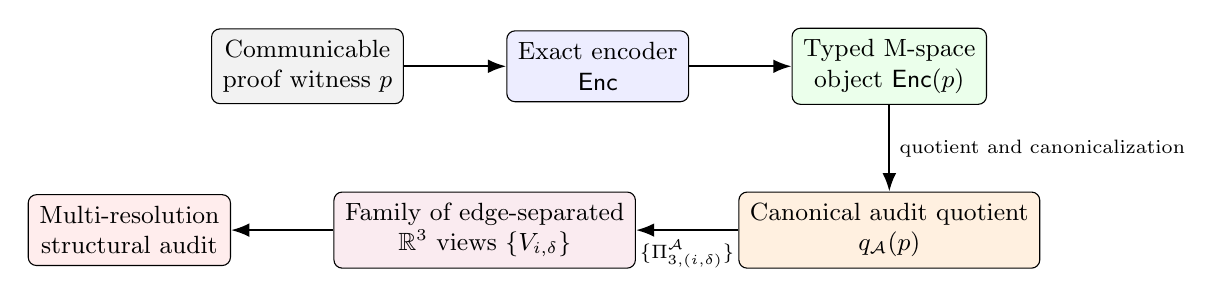
\begin{tikzpicture}[node distance=11mm and 13mm, >=Latex, every node/.style={font=\small}, box/.style={draw, rounded corners=3pt, align=center, minimum height=9mm, inner sep=4pt}, arrow/.style={->,thick}]
\node[box, fill=gray!10] (p) {Communicable\\proof witness $p$};
\node[box, fill=blue!7, right=of p] (enc) {Exact encoder\\$\Enc$};
\node[box, fill=green!8, right=of enc] (m) {Typed M-space\\object $\Enc(p)$};
\node[box, fill=orange!12, below=of m] (q) {Canonical audit quotient\\$\qA(p)$};
\node[box, fill=purple!8, left=of q] (v) {Family of edge-separated\\$\R^3$ views $\{V_{i,\delta}\}$};
\node[box, fill=red!7, left=of v] (h) {Multi-resolution\\structural audit};
\draw[arrow] (p)--(enc);
\draw[arrow] (enc)--(m);
\draw[arrow] (m)--node[right]{\scriptsize quotient and canonicalization}(q);
\draw[arrow] (q)--node[below]{\scriptsize $\{\Pi^{\mcA}_{3,(i,\delta)}\}$}(v);
\draw[arrow] (v)--(h);
\end{tikzpicture}
\caption{The proof-carrying representation cycle.  Exact representation preserves the source proof.  Quotienting removes only audit-irrelevant variation.  The display is in general a finite active record of $\R^3$ views indexed by
audit aspect $i$ and scale $\delta$; a finite admissible plan supplies the active
support and the local and global decoders.  For graph-shaped audit content, a
single member is a human-audit view only when it meets the declared interface
bound; \cref{thm:3d-preservation} remains the underlying geometric result.}
\label{fig:cycle}
\end{figure}

\subsection{The multi-resolution projection family}
\label{sec:family}

The general principle is not that a single rendering carries every distinction
in the quotient.  It is that a declared finite audit record carries the
distinctions required by the declared audit task at the aspects and scales that
are active for the proof under inspection.  A complete aspect--scale
decomposition determines what distinctions matter; a finite admissible plan
determines which finitely many coherent views and decoders expose them for a
particular proof.

\begin{definition}[Complete aspect--scale decomposition]
\label{def:aspects}
A \emph{complete aspect--scale decomposition} of an audit family $\mcA$ consists
of a finite set $I$ of subfamilies $\mcA_i\subseteq\mcA$ and a scale index set
$\Delta$, which may be infinite, such that
\[
  \mcA=\bigcup_{i\in I}\mcA_i.
\]
For each aspect $i$ and scale $\delta\in\Delta$, let $\qA[i,\delta]$ denote the
quotient of the restricted family $\mcA_i$ read at resolution $\delta$
(formally, $\mcA_i$ composed with a declared finite coarsening
$c_\delta$ of its outputs).  The decomposition is \emph{complete} when
\[
  p\eqA p'
  \quad\Longleftrightarrow\quad
  \forall (i,\delta)\in I\times\Delta\,
  [\qA[i,\delta](p)=\qA[i,\delta](p')].
\]
Thus the full indexed family separates exactly the $\eqA$-classes.
\end{definition}

\begin{remark}[Completeness is not finite auditability]
\label{rem:complete-not-finite}
Completeness specifies what the full family distinguishes.  It does not imply
that an auditor can traverse every member of that family.  When $\Delta$ is
infinite, finite audit requires a separate proof-dependent finite-support
condition.
\end{remark}

\begin{definition}[Finite admissible projection plan]
\label{def:selection}
Fix a complete aspect--scale decomposition of $\mcA$ and the auditor model
$\mcH$ of \cref{ass:h0}.  A \emph{finite admissible projection plan} $\sigma$
consists of the following declared data and obligations.

\begin{enumerate}[label=\textnormal{(P\arabic*)},leftmargin=2.8em]
\item \textbf{Finite active support.} A map
\[
  J_\sigma:\Prf\longrightarrow\Fin(I\times\Delta).
\]
Only the aspect--scale pairs in $J_\sigma(p)$ are active in the audit record of
$p$.

\item \textbf{Selected finite subcomplexes.} For every $p\in\Prf$ and every
$(i,\delta)\in J_\sigma(p)$, a finite labelled subcomplex
\[
  S^\sigma_{i,\delta}(\Enc(p))
\]
of the canonical audit representative.

\item \textbf{Rendered views and coherence.} For every active index,
\[
  V^\sigma_{i,\delta}(p)
  =
  \Pi_3\bigl(S^\sigma_{i,\delta}(\Enc(p))\bigr)\in\mcV.
\]
The plan declares a finite-interface budget $\beta$ and a predicate
$\Coh_{\mcH,\beta}$ such that
\[
  \Coh_{\mcH,\beta}\bigl(V^\sigma_{i,\delta}(p)\bigr)=1
\]
for every active index.  The predicate records the relevant per-view bounds,
including displayed vertex count, edge density, legend complexity, and any
required traversal restriction.

\item \textbf{Local recovery.} For every active index, a declared decoder
\[
  \Lambda^\sigma_{i,\delta}:\mcV\longrightarrow Q_{i,\delta}
\]
satisfies
\[
  \Lambda^\sigma_{i,\delta}\bigl(V^\sigma_{i,\delta}(p)\bigr)
  =
  \qA[i,\delta](p).
  \tag{P1}\label{eq:localdecode}
\]

\item \textbf{Global recovery from the finite record.} Define
\[
  \ViewRec_\sigma(p)
  =
  \left\{
  \left(
  i,\delta,
  V^\sigma_{i,\delta}(p),
  \Lambda^\sigma_{i,\delta}(V^\sigma_{i,\delta}(p))
  \right):
  (i,\delta)\in J_\sigma(p)
  \right\}.
\]
The plan supplies a global decoder $\Gamma_\sigma$ on such finite indexed
records satisfying
\[
  \Gamma_\sigma\bigl(\ViewRec_\sigma(p)\bigr)=\qA(p)
  \qquad(p\in\Prf).
  \tag{P2}\label{eq:globaldecode}
\]
\end{enumerate}

The equations \eqref{eq:localdecode} and \eqref{eq:globaldecode} are
admissibility obligations of the plan.  They are not inferred merely from
calling a selected subcomplex ``audit relevant.''
\end{definition}

\begin{warning}[Why the decoder obligations are necessary]
\label{warn:decoder}
Suppose that the audit family contains a nonconstant task and that a proposed
selection rule returns the same empty subcomplex for every proof.  The selected
subcomplex is finite and may be trivially renderable, but no decoder can recover
a nonconstant audit value from identical empty views.  Thus pointwise finiteness
and renderability alone do not establish preservation.
\end{warning}

\begin{theorem}[Audit-preserving finite projection record]
\label{thm:family-preservation}
Let $(\mcA_i)_{i\in I},\Delta$ be a complete aspect--scale decomposition of
$\mcA$ and let $\sigma$ be a finite admissible projection plan.  Then for every
$p\in\Prf$:
\begin{enumerate}[label=\textnormal{(\roman*)},leftmargin=2.6em]
\item $\ViewRec_\sigma(p)$ is finite;
\item every active $V^\sigma_{i,\delta}(p)$ is an edge-separated
$\R^3$ object satisfying the declared coherence bound;
\item every active local quotient is recovered exactly by
\eqref{eq:localdecode}; and
\item the full audit quotient is recovered from the finite indexed record:
\[
  \Gamma_\sigma(\ViewRec_\sigma(p))=\qA(p).
\]
\end{enumerate}
\end{theorem}

\begin{proof}
The set $J_\sigma(p)$ is finite by \textnormal{(P1)} of
\cref{def:selection}; hence the indexed record is finite.  Every active
subcomplex is finite and its moment-curve realization is edge-separated by
\cref{lem:momentcurve}; coherence is part of \textnormal{(P3)}.  Exact local
recovery is \eqref{eq:localdecode}, and global recovery is
\eqref{eq:globaldecode}.
\end{proof}

\begin{corollary}[Single-view graph case under the interface bound]
\label{cor:single-view}
Suppose $\mcA$ is graph-shaped, so that the typed labelled incidence graph of
the canonical audit representative determines $\qA(p)$.  If, for a given
$p\in\Prf$, the full labelled incidence graph satisfies the declared coherence
predicate, then there is a singleton-support admissible plan for $p$ whose sole
view recovers $\qA(p)$ exactly.

For arbitrary finite proof-dependency graphs, the moment-curve construction
still gives a single edge-separated $\R^3$ realization.  This geometric
existence statement does not imply that the realization lies within a fixed
finite-interface capability bound.
\end{corollary}

\begin{proof}
Take $I=\{*\}$, $\Delta=\{*\}$, $\mcA_*=\mcA$, $c_*=\operatorname{id}$, and
$J_\sigma(p)=\{(*,*)\}$.  Select the full typed incidence graph and apply
\cref{thm:3d-preservation}.  The hypothesis supplies coherence, and the
single-view decoder gives both \eqref{eq:localdecode} and
\eqref{eq:globaldecode}.
\end{proof}

\begin{remark}[Geometry versus bounded auditability]
\label{rem:geometry-vs-interface}
Every finite graph has an edge-separated straight-line realization in
$\Rthree$, whereas no fixed finite display budget contains all finite graphs.
The first fact is graph-theoretic; the second follows from unbounded graph size.
Thus a universal $\Rthree$ realization theorem and a bounded single-screen
audit theorem are distinct claims.  Standard graph-theoretic background is
available in \cite{Diestel2017}.
\end{remark}

\begin{definition}[Before/after audit comparison]
\label{def:beforeafter}
For an admissible operation $o$ on proof states (an inference step, a rewrite,
an instantiation, or in the physical setting an admissible dynamical operation)
and an active aspect--scale pair $(i,\delta)\in J_\sigma(p)$, the
\emph{before/after audit} inspects the pair
\[
  \bigl(V^\sigma_{i,\delta}(p),\, V^\sigma_{i,\delta}(o\cdot p)\bigr)
\]
and verifies that the displayed change is exactly the change $o$ is declared to
produce on aspect $i$ at scale $\delta$.  The operation passes the structural
audit when all active before/after checks and the global bindings of
\cref{def:structaudit} hold.
\end{definition}

\subsection{Why three dimensions are universally minimal}

\begin{theorem}[Universal display dimension theorem]
\label{thm:dimension}
Three is the least integer $d$ such that every finite proof-dependency graph can be represented by an edge-separated visual realization in $\R^d$.
\end{theorem}

\begin{proof}
Sufficiency for $d=3$ follows from \cref{lem:momentcurve}.

For necessity, consider the ordinary propositional proof discipline with the axiom instances
\[
  A_i=(p_i\to p_i),\qquad i=1,\ldots,5,
\]
and conjunction introduction.  Form a finite proof ledger that proves every $A_i$, and for every pair $i<j$ introduces the auxiliary lemma
\[
  B_{ij}=A_i\wedge A_j.
\]
The incidence subgraph consisting of the five $A_i$ vertices and the ten conjunction-introduction rule vertices contains a subdivision of $K_5$: the rule vertex for $B_{ij}$ subdivides the edge between $A_i$ and $A_j$.  This is a valid finite proof object; unused or redundantly retained certified lemmas do not invalidate a proof ledger.

If every finite proof-dependency graph admitted an edge-separated realization in $\R^2$, this subdivided $K_5$ would be planar, and contracting each subdivided edge would yield a planar embedding of $K_5$.  But a simple planar graph with $v\geq 3$ vertices has at most $3v-6$ edges.  For $K_5$, $v=5$ and $e=10>9=3v-6$, a contradiction.  Thus $d\neq 2$, and dimensions $0$ and $1$ fail a fortiori.  Hence the least universal dimension is $3$.
\end{proof}

\begin{corollary}[Exact sense in which 3D is necessary]
\label{cor:3dnecessary}
A universal visually unambiguous proof-audit system must have access to at least three Euclidean spatial dimensions whenever it is required to display arbitrary finite dependency graphs without non-geometric crossing conventions.  Individual planar proofs may use two dimensions; the necessity is for the universal class.
\end{corollary}

\begin{remark}[The two distinct roles of ``3D'']
\label{rem:two-roles-3d}
The number three enters this architecture in two logically separate ways, and conflating them produces an apparent overclaim.
\begin{enumerate}
    \item \textbf{Sufficiency and minimality for the universal incidence class} (\cref{lem:momentcurve}, \cref{thm:dimension}): $\R^3$ is exactly enough, and $\R^2$ is not enough, to host edge-separated realizations of \emph{every} finite dependency graph.
    \item \textbf{Necessity as a human-channel constraint} (\cref{sec:human}): an auditor restricted to the capability model can trace paths only in a rendered $\R^{\le 3}$ object.  Consequently any aspect of the audit that is to be \emph{humanly traced} must be exposed by some $\R^{\le 3}$ projection; an intrinsically higher-dimensional relationship is auditable by such a person only through its $3$D projections.
\end{enumerate}
Role~(1) is a theorem about graphs.  Role~(2) is a theorem about the capability model.  Together they yield the operative statement: \emph{human structural audit without specialist background proceeds through $3$D-realizable projections; for graph-shaped content one projection suffices, and for intrinsic-geometric content a family of projections is required.}  Neither role asserts the false claim that one $3$D view always recovers every audit-relevant feature of every object.
\end{remark}

\section{Background-independent structural audit}
\label{sec:human}

A theorem cannot establish unmodeled facts about the perceptual capacities of
every human individual.  It can establish that a representation requires no
theorem-specific mathematics beyond an explicitly stated finite-interface
capability model, and that, \emph{given} that model and a finite admissible
projection plan, the declared structural audit is sound and complete.

\begin{assumption}[Generic structural-auditor capability model $\mcH$]
\label{ass:h0}
An auditor in $\mcH$ can:
\begin{enumerate}
    \item distinguish finite node types, finite labels, and equality of displayed tokens;
    \item follow an edge-separated path in a three-dimensional display, and compare two such displays element by element (before/after);
    \item enumerate a finite graph by a supplied traversal order;
    \item apply a finite interface legend; and
    \item invoke a trusted terminating local proof kernel on a displayed inference certificate and record its accept/reject result.
\end{enumerate}
The auditor is not required to possess prior specialist knowledge of the proof's
subject matter or the source calculus beyond the finite legend and trusted
kernel interface.  The capability is intrinsically three-dimensional: items
(2)--(4) are operations on rendered objects in $\R^{\le 3}$, so the auditor has
no access to a distinction that no $\R^{\le 3}$ projection exposes.
\end{assumption}

\begin{remark}[$\mcH$ is a constraint, not a hedge]
\label{rem:h-constraint}
Because the auditor operates only on rendered $\R^{\le 3}$ objects, $\mcH$
makes explicit the constraint ``human-auditable $\Rightarrow$ exposed by a
coherent $3$D projection.''  It forces a projection plan for
intrinsic-geometric content: an aspect not exposed in any active coherent view
is, for an auditor in $\mcH$, unaudited.  It does not convert arbitrary finite
or arbitrarily dense displays into bounded human-interface objects.
\end{remark}

\begin{definition}[Plan-realized structural audit family]
\label{def:plan-realized}
Let $\sigma$ be a finite admissible projection plan for
$\mcA_{\mathrm{str}}$.  The family $\mcA_{\mathrm{str}}$ is
\emph{plan-realized} when every declared structural task has a finite acceptance
procedure determined by:
\begin{enumerate}[label=\textnormal{(\roman*)},leftmargin=2.6em]
\item the finite decoded record $\Gamma_\sigma(\ViewRec_\sigma(p))$;
\item the locally decoded values
$\Lambda^\sigma_{i,\delta}(V^\sigma_{i,\delta}(p))$;
\item the finite traversal data displayed in the active views; and
\item the accept/reject outputs of the declared trusted local proof kernel.
\end{enumerate}
This is not a claim of semantic soundness for an arbitrary calculus.  It
requires only that the declared structural tasks be checkable through the
specified finite trusted interface.
\end{definition}

\begin{definition}[Structural audit]
\label{def:structaudit}
Given a finite admissible plan $\sigma$ and a proof $p$, a
\emph{structural audit} is the finite procedure that:
\begin{enumerate}
    \item reads the finite indexed record $\ViewRec_\sigma(p)$ and its active
    support $J_\sigma(p)$;
    \item for each $(i,\delta)\in J_\sigma(p)$, traverses every displayed vertex
    and edge of $V^\sigma_{i,\delta}(p)$ once according to the supplied audit
    order;
    \item checks that the displayed conclusion, calculus identifier, and stated
    audit target agree with the decoded record;
    \item checks each displayed inference's ordered premise binding and invokes
    the local kernel;
    \item checks that every certificate and external assumption has a declared
    status and provenance edge, and that each active before/after change matches
    the declared operation; and
    \item computes the local values and
    $\Gamma_\sigma(\ViewRec_\sigma(p))$, outputting \textsf{pass} precisely when
    all required local checks, active-view checks, and global bindings pass.
\end{enumerate}
\end{definition}

\begin{theorem}[General-background structural audit theorem, corrected conditional form]
\label{thm:human-audit}
Fix a complete aspect--scale decomposition of $\mcA_{\mathrm{str}}$, a finite
admissible projection plan $\sigma$, and the capability model $\mcH$.  Assume
that $\mcA_{\mathrm{str}}$ is plan-realized in the sense of
\cref{def:plan-realized} and that the local proof kernel terminates on every
certificate presented by the plan.  Then every $p\in\Prf$ admits a finite
structural audit, and the audit passes if and only if every declared task in
$\mcA_{\mathrm{str}}$ accepts on $p$.
\end{theorem}

\begin{proof}
The active support $J_\sigma(p)$ is finite, and every active view is finite and
satisfies its declared coherence bound.  Hence every required display traversal
and comparison is a finite operation available to an auditor in $\mcH$.  The
local kernel invocations terminate by hypothesis.  Equations
\eqref{eq:localdecode} and \eqref{eq:globaldecode} recover the local task values
and the full audit quotient from the finite record.  The plan-realization
condition therefore supplies exactly the information used by each declared
structural task.  Consequently the audit passes exactly when every such task
accepts.
\end{proof}

\begin{remark}[Corrected scope]
\label{rem:disclaimer-to-hyp}
What is a theorem is: \emph{given} the capability model $\mcH$, a finite
admissible projection plan, a plan-realized task family, and a terminating local
kernel, the audit is sound and complete.  What is not a theorem is that an
arbitrary large or dense rendering is humanly auditable, that every selection
rule has the decoders required for preservation, or that an infinite
aspect--scale family is automatically traversable in finitely many operations.
\end{remark}

\begin{remark}[What ``without specific mathematical backgrounds'' means]
\label{rem:background}
The theorem does not say that a person with no mathematical education suddenly
understands every concept in algebraic geometry, set theory, or higher category
theory.  It says that the \emph{structural validity audit} of the represented
proof does not require theorem-specific background knowledge once the source
calculus is reduced to a trusted local checker and the interface grammar is
finite.  Semantic interpretation of a field's concepts may require further
education; representation integrity, dependency tracing, certificate checking,
and before/after comparison do not.  It is exactly because the non-specialist
cannot supply missing features from background knowledge that those features
must be made visible in the finite active record that pins them down.
\end{remark}

\subsection{Maximal auditability in the formal sense}

For a fixed audit family, ``maximally auditable'' means complete discrimination with no irrelevant discrimination burden.

\begin{definition}[Audit burden preorder]
\label{def:burden}
For audit-faithful representations $r_1:\Prf\to R_1$ and $r_2:\Prf\to R_2$, write
\[
  r_1\preceq_{\mcA} r_2
\]
when there exists $u:\Img(r_2)\to\Img(r_1)$ such that $r_1=u\circ r_2$.  Thus $r_2$ retains at least every distinction retained by $r_1$.  A representation has lower audit discrimination burden when it is lower in this preorder while remaining audit-faithful.
\end{definition}

\begin{corollary}[Quotient-optimal general audit]
\label{cor:maxaud}
The canonical quotient representation $\qA$ is least in the audit burden preorder among all $\mcA$-faithful representations.  Under a finite admissible projection plan, its finite active three-dimensional record is complete for the declared audit task while carrying no audit-irrelevant distinction.  A graph-shaped record is a single human-audit view only under the plan's interface bound.  Combined with \cref{thm:dimension}, this yields the precise joint statement of minimum necessary task distinction and minimum universal edge-separated display dimension, without identifying geometric universality with unbounded screen auditability.
\end{corollary}

\begin{proof}
\Cref{thm:coarsest} gives $\qA=h_r\circ r$ for every audit-faithful $r$, which is exactly $\qA\preceq_{\mcA} r$.  \Cref{thm:family-preservation} transfers this quotient without loss to the finite
active record, while \cref{thm:3d-preservation} gives the underlying
graph-shaped geometric singleton.  \Cref{thm:dimension} proves minimal universal
display dimension.
\end{proof}


\section{Collective proof-audit capacity and the empirical bridge}
\label{sec:collective-capacity}

The universal M-space results establish what a representation must preserve for a
specified audit task.  They do not alone establish whether a distributed
mathematical community has enough time, personnel, or interface support to apply
that audit as new proof-relevant artifacts arrive.  This section separates a
formal accounting theorem from the empirical bridge required to instantiate it.
The observable object is deliberately a source-visible proof-audit ledger, not
``mathematics as a whole.''

\subsection{Time-indexed proof-audit ledger}

\begin{definition}[Time-indexed proof-audit ledger]
\label{def:ledger}
For discrete windows $t\in\N$, a proof-audit ledger is
\[
  \Ledger_t=(V_t,E_t,O_t,R_t,\tau_t).
\]
$V_t$ is the finite set of versioned proof-relevant artifacts; $E_t$ is a finite
typed relation set; $O_t\subseteq V_t$ is the unresolved audit-item set; $R_t$
is the set of recorded resolution events; and $\tau_t$ records source version,
retrieval time, and extraction provenance.  When the source supports the
distinction, relation types include dependency, import, reference, review,
challenge, repair, supersession, and resolution.
\end{definition}

\begin{remark}[Ledger boundary]
\label{rem:ledger-boundary}
An absent edge can mean absence of a relation, an unobserved relation, or a
relation not expressible in the selected source.  Thus the ledger cannot be used
as a census of mathematical activity, a ranking of researchers, or a direct
measure of mathematical truth.  It is an explicit, reproducible record of the
subset of proof-relevant artifacts and relations that a declared source exposes.
Formal libraries make a useful primary domain precisely because they publish
versioned declarations, dependencies, builds, and repair histories
\cite{mathlib2020,vanDoorn2020,blanchette2015,huch2024}.
\end{remark}

\subsection{Demand, capacity, debt, and cost monotonicity}

\begin{definition}[Audit-work accounting]
\label{def:accounting}
Fix an audit family $\mcA$ and an $\mcA$-faithful representation $r$.  Let
$A_t$ be the finite set of obligations opened or reopened in window $t$; let
$c_r(o)\in\R_{\geq0}$ be the declared work to resolve $o$ through $r$; and let
$\AuditCap_t\in\R_{\geq0}$ be the available audit capacity.  Set
\[
  \Demand_r(t)=\sum_{o\in A_t}c_r(o),\qquad
  \Debt_{r,t+1}=\max\{0,\Debt_{r,t}+\Demand_r(t)-\AuditCap_t\}.
  \tag{C1}\label{eq:debt}
\]
The work unit can be clock time, verified traversal steps, or a predeclared
weighted item count.  It must be fixed before observing outcomes when the
accounting is used empirically.
\end{definition}

\begin{remark}[Reflected workload recurrence]
The update in \eqref{eq:debt} is a deterministic reflected workload recurrence.
It is structurally analogous to the recurrence introduced by Lindley for a
single-server queue \cite{Lindley1952}, but no stochastic arrival, service, or
stationarity premise is used here.
\end{remark}

\begin{assumption}[Audit-cost monotonicity]
\label{ass:cost}
For $\mcA$-faithful representations $r_1$ and $r_2$, if
$r_1=u\circ r_2$ for some $u:\Img(r_2)\to\Img(r_1)$, then
\[
  c_{r_1}(o)\leq c_{r_2}(o)
\]
for every obligation $o$ in the declared domain.  In other words, preserving
an additional distinction cannot lower the stipulated structural-audit work when
that distinction is irrelevant to every task in $\mcA$.
\end{assumption}

\begin{remark}[Why this is an assumption]
\label{rem:cost-assumption}
The quotient theorem alone orders information, not human minutes or institutional
budgets.  \Cref{ass:cost} is the bridge from information order to a work order.
It is appropriate for a formal theorem because it is explicit and falsifiable as
a model of the stated audit process; it is not an unrestricted claim that every
compression reduces every person's cognitive effort.
\end{remark}

\begin{theorem}[Persistent demand-capacity excess yields unbounded debt]
\label{thm:debt}
Fix $r$.  If there are $t_0\in\N$ and $\varepsilon>0$ such that
\[
  \Demand_r(t)-\AuditCap_t\geq\varepsilon
  \qquad(t\geq t_0),
\]
then
\[
  \Debt_{r,t}\geq\Debt_{r,t_0}+(t-t_0)\varepsilon
  \qquad(t\geq t_0),
\]
and therefore $\Debt_{r,t}\to\infty$.
\end{theorem}

\begin{proof}
By \eqref{eq:debt},
$\Debt_{r,t+1}\geq\Debt_{r,t}+\varepsilon$ for every $t\geq t_0$.
Induction gives the displayed inequality.
\end{proof}

\begin{theorem}[Audit-quotient capacity dominance]
\label{thm:capacity}
Under \Cref{ass:cost}, the audit quotient $\qA$ satisfies
\[
  \Demand_{\qA}(t)\leq\Demand_r(t)
  \qquad\text{for every $\mcA$-faithful $r$ and every $t$.}
  \tag{C2}\label{eq:dominance}
\]
For equal initial debt and a common capacity schedule,
\[
  \Debt_{\qA,t}\leq\Debt_{r,t}
  \qquad(t\in\N).
  \tag{C3}\label{eq:debt-dominance}
\]
Suppose that $r$ has a persistent positive demand-capacity excess while
\[
  \Demand_{\qA}(t)-\AuditCap_t\leq0
  \qquad(t\geq t_0)
  \tag{C4}\label{eq:quotient-within-capacity}
\]
for some $t_0$.  Then replacement of $r$ by the audit quotient is a sufficient
representation-level repair: quotient debt is nonincreasing after $t_0$, while
the debt of $r$ diverges.

More generally, any proposed repair that avoids the divergence conclusion must
change at least one antecedent of \cref{thm:debt}: the
representation-specific demand, the capacity schedule, the incoming obligation
process, the declared audit domain or task, or the persistence condition.  This
does not assert that every successful repair must literally use the quotient
realization.
\end{theorem}

\begin{proof}
By \Cref{thm:coarsest}, $\qA=h_r\circ r$ on $\Img(r)$.  The cost inequality in
\Cref{ass:cost} gives $c_{\qA}(o)\leq c_r(o)$ itemwise, and summation gives
\eqref{eq:dominance}.  The update map
$x\mapsto\max\{0,x\}$ is monotone, so induction in \eqref{eq:debt} gives
\eqref{eq:debt-dominance}.  Under \eqref{eq:quotient-within-capacity},
\[
  \Debt_{\qA,t+1}\leq\Debt_{\qA,t}
  \qquad(t\geq t_0).
\]
If $r$ has persistent excess, \cref{thm:debt} gives divergence.  The final
statement follows because that divergence theorem depends only on its displayed
recurrence and antecedent conditions; another successful repair may alter one of
them without literally adopting the quotient.
\end{proof}

\begin{corollary}[Conditional collective coherence criterion]
\label{cor:collective}
For a fixed ledger, audit family, work model, and capacity schedule, the audit
quotient maximizes the formal margin $\AuditCap_t-\Demand_r(t)$ among
$\mcA$-faithful representations.  Hence a persistent loss of that margin is not
repaired by adding audit-irrelevant representational distinctions.  This
dominance does not make the quotient the literal only representation through
which a workflow can avoid debt.
\end{corollary}

\begin{proof}
Immediate from \eqref{eq:dominance}.
\end{proof}

\subsection{Preregistered empirical bridge}

The preceding results are not observational claims.  They say what follows
\emph{if} a ledger, capacity schedule, and cost monotonicity model are correctly
declared.  The empirical bridge is therefore stated as a separate preregistered
protocol rather than silently treated as a theorem premise
\cite{nosek2018}.  Its primary domain is source-visible formal mathematics,
not informal citation volume.

\begin{definition}[Candidate source-visible coherence bottleneck]
\label{def:bottleneck}
Let $I_t$ be the unweighted count of newly opened audit items, $K_t$ the
unweighted count of recorded resolution events, and
$\rho_t=I_t/K_t$ when $K_t>0$.  For an undirected analysis backbone
$\overline G_t$, let $\lambda_2(t)$ be the second normalized-Laplacian
eigenvalue.  A window interval $[t,t+m-1]$ is a candidate source-visible
coherence bottleneck when, under a frozen extraction manifest:
\begin{enumerate}[label=(\roman*),leftmargin=.75cm]
  \item $m\geq3$ consecutive active windows have $\rho_j>1$;
  \item $\Debt_{t+m-1}\geq1.25\Debt_t$ under the protocol's fixed accounting;
  \item $\lambda_2$ is below the corpus's trailing four-window median; and
  \item no declared source outage, bulk import, or migration explains more than
  $50\%$ of the relevant inflow.
\end{enumerate}
This is an operational alert condition, not a diagnosis that a mathematical
field is false, fragmented in every relevant sense, or socially dysfunctional.
\end{definition}

\begin{remark}[Graph boundary]
\label{rem:graph-boundary}
Algebraic connectivity and conductance are standard structural graph measures
\cite{fiedler1973,chung1997}.  In this architecture they are features for a
forecasting test, not truth values.  Bibliographic graphs may supply secondary
communication triangulation, but they neither validate a proof nor replace
formal dependency and build evidence.
\end{remark}

\begin{hypothesis}[Preregistered bridge hypotheses]
\label{hyp:bridge}
A complete empirical test should preregister at least the following separable
claims:
\begin{enumerate}[label=\textnormal{(E\arabic*)},leftmargin=2.4em]
\item A ledger-feature model improves locked-test forecasting of a future
audit-debt event over a workload-only baseline in at least one formal corpus and
has nonnegative direction in an independent corpus.
\item The finding does not disappear under source-outage, scale, bulk-import,
time-shuffle, and degree-preserving graph-rewire controls.
\item On bounded structural-audit tasks, a task-faithful audit-quotient display
outperforms a text/list baseline in preregistered accuracy or time outcomes
without serious usability harm.
\item A linked $3$D view is tested against a linked $2$D quotient view with an
expertise interaction; it is not assumed to be superior, and a general-background
advantage is claimed only if its interval estimate is positive without a
predeclared usability penalty.
\end{enumerate}
\end{hypothesis}

A suitable primary corpus pair is Lean \texttt{mathlib} and the Archive of
Formal Proofs; each exposes a different formal-library workflow and therefore
makes a nontrivial replication target \cite{mathlib2020,vanDoorn2020,
blanchette2015,huch2024}.  The interface experiment compares: text/list
records; a static $2$D dependency display; an audit quotient with linked $2$D
views; and the same quotient with a controllable $3$D view plus $2$D fallback.
The task is bounded structural audit (certificate availability, dependency-path
interruption, minimum repair object, or task-relative audit equivalence), never
a request that a non-specialist establish the semantic truth of an advanced
theorem.  These protocol restrictions preserve the distinction between
\Cref{thm:human-audit}'s conditional formal auditor and actual human outcomes.

\begin{remark}[Falsification and status]
\label{rem:emp-falsification}
Failure of the locked-test improvement, replication direction, quotient interface
advantage, or $3$D-versus-$2$D usability criterion counts against the corresponding
empirical bridge hypothesis, not against the quotient or dimension theorems.
Conversely, a positive study does not prove that every mathematical domain has
a coherence bottleneck or that $3$D is universally optimal.  The correct status
is $\mathsf{EMP}$: a preregistered, testable empirical proposition.
\end{remark}

\section{P-space: the same architecture for physics}
\label{sec:pspace}

The construction above used nothing about $\Prf$ beyond: a class of finitely communicable typed objects, a family of audit tasks, a local trusted checker, and a typed incidence structure.  Physical state spaces (P-space) supply exactly these ingredients, with admissible dynamical operations in place of inference rules.  This section states the transfer and identifies precisely where physics differs from proof-dependency audit --- namely, that its audit content is intrinsic-geometric, so the projection family is genuinely multi-membered.

\begin{definition}[P-space audit object]
\label{def:pspace}
A \emph{P-space audit object} for a bounded region $R$ at description resolution $\delta$ is a finite typed object
\[
  P(R,\delta)=(G,\,L_0,\ldots,L_n)
\]
of the same M-tower form as \cref{def:mtower}, where $G$ is a finite typed graph of physical state elements and admissible-operation vertices, $L_0$ stores the exact finite state description at resolution $\delta$, and the higher layers carry normalized physical quantities, local conservation/transition certificates, provenance, and display obligations.  Admissible operations are the declared dynamical compositions (e.g.\ interaction vertices) whose local certificates a trusted physical checker can verify.
\end{definition}

\begin{definition}[Interaction-aspect decomposition]
\label{def:interaction-aspects}
For P-space the aspect index set is the set of admissible interaction channels,
\[
  I=\{\text{strong},\ \text{weak},\ \text{electromagnetic},\ \text{gravitational},\ \text{(composed channels)}\},
\]
and $\Delta$ is the set of physical scales.  For each $(i,\delta)$, $\mcA_i$ at scale $\delta$ is the family of audit tasks that determine the transition produced by interaction $i$ at scale $\delta$.
\end{definition}

\begin{remark}[Why P-space needs the family and cannot collapse to one view]
\label{rem:pspace-family}
In proof-dependency audit the whole quotient is graph-shaped, so a
singleton-support plan is available whenever the full incidence display meets
the declared interface bound (\cref{cor:single-view}).  Physics is different:
the relations that determine a strong-interaction transition at one scale, a
weak transition at another, and electromagnetic or gravitational structure at
others are not jointly readable from one incidence picture.  The correct
architecture is therefore a finite admissible projection plan of
\cref{sec:family}: for each proof object it selects a finite active support of
interaction--scale views and supplies the decoders that reconstruct the declared
physical audit quotient.  The active before/after comparisons have the form
\[
  V^\sigma_{i,\delta}\bigl(P_{\text{before}}(R,\delta)\bigr)
  \ \longrightarrow\
  V^\sigma_{i,\delta}\bigl(P_{\text{after}}(R,\delta)\bigr),
  \qquad (i,\delta)\in J_\sigma(P).
\]
No single rendering carries every physically relevant distinction
simultaneously, and none needs to.
\end{remark}

\begin{theorem}[P-space audit architecture]
\label{thm:pspace}
Let $P(R,\delta)$ be a P-space audit object for a bounded region, let
$(\mcA_i)_{i\in I},\Delta$ be a complete interaction-aspect decomposition of its
physical audit family, and let $\sigma$ be a finite admissible projection plan.
Assume that the declared physical audit family is plan-realized and that its
trusted local checker terminates on every certificate presented by the plan.
Then:
\begin{enumerate}
    \item $P(R,\delta)$ has an exact M-tower representation with a lossless decoder (transfer of \cref{thm:universal-representation});
    \item the physical audit quotient $\qA$ is the coarsest representation preserving the declared physical audit family (transfer of \cref{thm:coarsest});
    \item the finite active interaction/scale record consists of edge-separated $\R^3$ objects and preserves the quotient through the plan's local and global decoders (transfer of \cref{thm:family-preservation});
    \item under \cref{ass:h0}, an auditor can perform a finite, sound-and-complete before/after structural audit of the declared active interaction/scale tasks (transfer of \cref{thm:human-audit}); and
    \item three remains the least Euclidean dimension universally sufficient for edge-separated rendering of the finite interaction-incidence graphs; any claim that a single physical view is auditable additionally requires its declared interface bound.
\end{enumerate}
\end{theorem}

\begin{proof}
Each clause is the cited M-space theorem applied to the P-space audit object,
whose defining data (finite typed objects, a physical audit family, a trusted
local checker, a typed interaction-incidence structure, and admissible
operations) instantiate the hypotheses used in each proof.  The structural
difference from the proof case is that the audit content is
intrinsic-geometric rather than graph-shaped, so the plan generally has a
multi-member active support.  This changes the plan supplied to
\cref{thm:family-preservation} but not the conditional transfer.
\end{proof}

\section{Reliable derivation and novelty-separated domains}
\label{sec:necessity}

\subsection{Derivational tasks}

A representation theorem must not be conflated with a universal theorem-discovery algorithm.  The following definition captures the correct object: a procedure is reliable when it produces correct derivational or audit decisions on its declared domain, not when it decides all mathematical truth.

\begin{definition}[Derivational decision problem]
\label{def:derivproblem}
A \emph{derivational decision problem} is a triple
\[
  \mathfrak D=(X,T,\mathcal R),
\]
where $X\subseteq\Prf$ is a declared class of proof states or proof-search states, $T:X\to Y$ is the decision required for reliable derivation or audit, and $\mathcal R$ is a family of permitted representation channels $r:X\to R_r$.

A procedure based on $r$ is \emph{reliable for $T$ on $X$} if there exists $d_r:R_r\to Y$ such that
\[
  T=d_r\circ r.
\]
This includes proof validation, next-step selection, branch elimination, obligation tracking, and any other declared derivational target.  It does not require a total algorithm deciding theoremhood outside the declared domain.
\end{definition}

\begin{definition}[Novelty separation]
\label{def:novelty}
The problem $\mathfrak D=(X,T,\mathcal R)$ is \emph{novelty-separated relative to $\mathcal R$} when
\[
  \forall r\in\mathcal R\;\exists x,y\in X
  \quad r(x)=r(y)\ \text{and}\ T(x)\neq T(y).
\]
Write $\Novel(X,T;\mathcal R)$ for this condition.
\end{definition}

This is a formal replacement for vague claims of ``sufficient novelty.''  A domain is sufficiently novel relative to a representational repertoire exactly when the repertoire has not yet preserved the distinctions needed by the derivational task.

\begin{theorem}[Representation-necessity theorem]
\label{thm:necessity}
Let $\mathfrak D=(X,T,\mathcal R)$ be a novelty-separated derivational decision problem.  Then no procedure using only a channel $r\in\mathcal R$ is reliable for $T$ on $X$.
\end{theorem}

\begin{proof}
Fix $r\in\mathcal R$.  By novelty separation, choose $x,y\in X$ with $r(x)=r(y)$ and $T(x)\neq T(y)$.  If a reliable procedure $d_r$ existed, then
\[
T(x)=d_r(r(x))=d_r(r(y))=T(y),
\]
a contradiction.
\end{proof}

\begin{theorem}[M-space-equivalent necessity]
\label{thm:mnecessary}
Let $X\subseteq\Prf$ and let $\mcA$ be the audit family required for a reliable derivation workflow.  If a representation $r:X\to R$ supports reliable completion of every task in $\mcA$, then the restricted audit quotient factors through $r$:
\[
  \qA|_X=h_r\circ r
\]
for a unique map $h_r$ on $\Img(r)$.  Hence every reliable workflow must retain an M-space-equivalent refinement of
the audit quotient.  If the workflow must also present an edge-separated,
general-background visual audit of arbitrary finite proof-dependency graphs,
then it requires a representation with a three-dimensional visual factor, up to
audit equivalence.  A single graph display is a human-audit factor only when it
meets the declared interface bound; for intrinsic-geometric content the factor
is in general a finite admissible family of three-dimensional views rather than
a single view.
\end{theorem}

\begin{proof}
The first statement is \cref{thm:coarsest} applied to the restricted domain
$X$.  The M-space encoder and visual projection realize $\qA|_X$ by
\cref{thm:universal-representation} and \cref{thm:family-preservation}.  If a
general-background visual audit is required for arbitrary finite
proof-dependency graphs, any universal edge-separated realization in dimension
below three is impossible by \cref{thm:dimension}; and by
\cref{rem:two-roles-3d} an auditor in $\mcH$ accesses a distinction only if some
$\R^{\le3}$ projection exposes it.  Thus the reliable workflow must preserve the
quotient information and offer at least a three-dimensional equivalent visual
factor under the stated interface requirement.  The finite admissible plan
collapses to one view only for graph-shaped content whose full selected display
satisfies its declared bound (\cref{cor:single-view}).
\end{proof}

\begin{corollary}[Novel-domain derivational audit]
\label{cor:novel-audit}
Suppose $\Novel(X,T;\mathcal R)$ holds, and suppose $T$ includes the full structural audit tasks $\mcA_{\mathrm{str}}$ required to distinguish the witness pairs produced by the available channels.  Then no member of $\mathcal R$ can support a reliably correct derivational
audit.  An M-space (or P-space) representation $\Enc$ followed by a
quotient-preserving finite admissible projection plan supplies a sufficient
enriched channel, provided the local checker, declared task bridges,
plan-realization condition, and terminating local kernel are available.
\end{corollary}

\begin{proof}
Non-adequacy of $\mathcal R$ follows from \cref{thm:necessity}.  Sufficiency of the constructed enriched channel follows from exact
representation, quotient preservation, and the structural audit theorem
(\cref{thm:human-audit}), under the stated finite-plan hypotheses.
\end{proof}

\begin{remark}[Necessity is invariant, not a demand for a literal file format]
\label{rem:equivnecessity}
If $b$ is a bijection on representation tokens, then $b\circ\Enc$ is as faithful as $\Enc$.  Therefore no mathematical theorem can establish that a reliable process must use the literal letters ``M-space,'' a particular drawing program, or a particular data format.  What is forced is the invariant content: a representation that refines the
required audit quotient and, when universal edge-separated human tracing is part
of the task, has an audit-equivalent three-dimensional factor realized by the
declared finite plan (one view only when the graph-shaped display meets its
interface bound).  This invariance is not a hedge to be removed; it is a
theorem, and it is the precise reason the ``literal-format superiority'' entry
below is correctly classified as not a theorem.
\end{remark}

\section{The assembled full architectural theorem}
\label{sec:assembled}

\begin{theorem}[Universal M-space proof architecture theorem]
\label{thm:full}
Let $\Prf$ be the class of communicable purely mathematical proof witnesses from
\cref{def:proof}.  Let $\M_\infty$ be the M-space proof tower from
\cref{def:mtower}.  Let $\mcA_{\mathrm{str}}$ be the full structural audit
family, fixed together with a complete aspect--scale decomposition, a finite
admissible projection plan $\sigma$, and the generic structural-auditor
capability model $\mcH$ from \cref{ass:h0}.  Assume that
$\mcA_{\mathrm{str}}$ is plan-realized and that the local kernel terminates on
every certificate presented by $\sigma$.  Then:
\begin{enumerate}
    \item \textbf{Universal proof representation.} Every $p\in\Prf$ has an exact representation $\Enc(p)\in\M_{N(p)}$ for some finite $N(p)$, and $\Dec\circ\Enc=\operatorname{id}_{\Prf}$.
    \item \textbf{Audit-optimal compression.} The quotient $\qA$ is the coarsest representation preserving every full structural audit task.  Every other audit-faithful representation retains a refinement from which $\qA$ is recoverable.  No absolute bit-length dominance is claimed, because none exists (\cref{prop:no-abs}).
    \item \textbf{Finite three-dimensional audit record.} For every $p$, the plan yields a finite indexed record $\ViewRec_\sigma(p)$ of edge-separated labelled $\R^3$ objects whose local and global decoders recover $\qA(p)$.  For graph-shaped content, this record is a singleton only when the full labelled incidence display satisfies the declared interface bound.
    \item \textbf{Three-dimensional universal minimality.} No Euclidean dimension below three admits an edge-separated visual realization of every finite proof-dependency graph, while three does.  This universal geometric fact is distinct from a bounded single-view human-audit claim.
    \item \textbf{Background-independent structural audit, conditional form.} Given $\mcH$, $\sigma$, plan-realization, and a terminating local kernel, every $p$ admits a finite sound-and-complete structural audit of the displayed record without theorem-specific mathematical background beyond the finite legend and trusted local kernel.
    \item \textbf{Necessity in novelty-separated derivational domains.} If the available representation family collapses states on which the required derivational/audit target differs, no procedure using only that family is reliable.  Any reliable replacement must retain an audit-equivalent refinement of $\qA$; and if its required audit is universal, edge-separated, and general-background visual, it must admit an audit-equivalent three-dimensional factor realized by the declared finite plan.
    \item \textbf{Collective proof-audit capacity.} Given the ledger accounting and
cost monotonicity, the audit quotient weakly minimizes incoming audit demand and
therefore maximizes the formal capacity margin among faithful representations.
A persistent positive demand-capacity excess produces unbounded debt.  When the
quotient has nonpositive excess, quotient replacement is a sufficient
representation-level repair; other repairs are not excluded if they alter a
stated premise of the recurrence.
    \item \textbf{Cross-domain transfer.} Clauses (1)--(7) hold in the stated
conditional form for P-space audit objects (\cref{thm:pspace}), with a generally
multi-member finite active record because physical audit content is
intrinsic-geometric.
\end{enumerate}
\end{theorem}

\begin{proof}
Items (1)--(6) are respectively
\cref{thm:universal-representation,thm:coarsest,thm:family-preservation,thm:dimension,thm:human-audit,thm:mnecessary}, with (2) supplemented by
\cref{prop:no-abs} and (3) specialized by \cref{cor:single-view}; item (7) is
\cref{thm:capacity}; and item (8) is \cref{thm:pspace}.  Their compatibility
follows because the encoder, quotient, finite projection record, decoders,
auditor, and capacity accounting are connected by
\eqref{eq:localdecode}, \eqref{eq:globaldecode}, and \eqref{eq:dominance}.
No item promotes representation to semantic truth, task-relative compression to
absolute code-length dominance, a formal auditor model to unmodeled empirical
psychology, or an accounting theorem to an empirical diagnosis.  The finite
support, decoders, plan-realization condition, auditor model, and empirical
bridge appear explicitly where required.
\end{proof}

\section{Application bridge templates and falsifiers}
\label{sec:bridges}

\begin{definition}[Bridge completion template]
For any external use, supply:
\[
\mathsf{Bridge}_{\mathrm{app}}=
(X_{\mathrm{app}},\iota,T_{\mathrm{app}},o_{\mathrm{app}},
\Psi_{\mathrm{app}},\mathcal R,\mathcal E,\Status).
\]
The completion must identify:
\begin{enumerate}[label=\textnormal{(B\arabic*)},leftmargin=2.6em]
\item the application state carrier and its intended domain;
\item the propagation law or data-generating update;
\item the actual observation channel available to the specified assessor;
\item the intended orbit predicate and its measurement/semantic bridge;
\item either a descent decoder or a finite paired non-descent witness;
\item unresolved assumptions and modeled approximation errors; and
\item a finite class of observations that would defeat the proposed bridge.
\end{enumerate}
\end{definition}

\begin{remark}[No policy propagation]
A $\DTwo$ status can block an inference from a declared channel to a declared
tail target.  It does not by itself prescribe intervention, withdrawal,
continuation, policy, or a physical conclusion.  Such an action requires its own
objective function, constraints, uncertainty model, and authorization rule.
\end{remark}

\begin{longtable}{p{0.10\textwidth}p{0.54\textwidth}p{0.22\textwidth}}
\caption{Claim-status ledger for Version 11.}\label{tab:claim-status}\\
\toprule
ID & Claim & Status \\
\midrule
\endfirsthead
\toprule
ID & Claim & Status \\
\midrule
\endhead
C1 & Fiber criterion and paired non-descent consequence & $\mathsf{THM}$ \\
C2 & Rich temporal witness and history-derived non-repair & $\mathsf{THM}$ \\
C3 & Coarsest decision partition & $\mathsf{THM}$ \\
C4 & Wall-valued separation; Boolean collapse limitation & $\mathsf{THM}$ \\
C5 & Record-level $\DOne/\DTwo/\DThree$ soundness & $\mathsf{THM}$ \\
C6 & Binding-sensitive non-factorization relative to $\pi_{\mathrm{cmp}}$ & $\mathsf{THM}$ \\
C7 & $\UGapTail\leftrightarrow\ACA$ over $\RCA$ & $\mathsf{THM}$ \\
M1 & Exact M-space representation and decoding of communicable proof witnesses & $\mathsf{THM}$ \\
M2 & Audit-quotient optimal compression relative to a declared audit family & $\mathsf{THM}$ \\
M3 & Universal edge-separated $\mathbb R^3$ realization and dimension minimality for finite proof-dependency graphs & $\mathsf{THM}$ \\
M4 & General-background structural audit under the declared auditor model, finite admissible projection plan, plan-realization condition, and terminating local kernel & $\mathsf{CND}$ \\
M5 & Necessity of an audit-equivalent refinement in novelty-separated derivational domains & $\mathsf{THM}$ \\
M6 & Ledger debt divergence and quotient-capacity dominance under declared accounting and cost monotonicity & $\mathsf{THM}/\mathsf{CND}$ \\
M7 & P-space/A(R)-space invariant-level correspondence or physical instantiation & $\mathsf{CND}/\mathsf{BR}$ \\
E1 & Formal-corpus forecasting and bounded human-audit interface hypotheses & $\mathsf{EMP}$ preregistered \\
A1 & Any institutional, ecological, AI, or physical instantiation & $\mathsf{BR}$ \\
P1 & Any action recommendation, physical bound, or policy conclusion & $\mathsf{OUT}$ from the formal core \\
\bottomrule
\end{longtable}

\begin{enumerate}[label=\textbf{F\arabic*.},leftmargin=2.6em]
\item An application bridge fails when its stated propagation, observation, or
predicate correspondence fails on the declared domain.
\item The exact M-space encoder claim fails if a finite accepted proof witness
cannot be encoded at a finite tower level or fails exact decoding.
\item The audit-optimal quotient claim fails if an audit-faithful representation
identifies two proof witnesses separated by the declared audit quotient.
\item The universal three-dimensional minimality claim fails if every finite
proof-dependency graph has an edge-separated realization in $\mathbb R^2$, or if
some finite graph lacks the stated $\mathbb R^3$ realization.  Claims concerning human structural audit remain conditional on the stated
capability model, finite admissible projection plan, plan-realization condition,
and terminating local kernel.
\item The collective-capacity theorem is inapplicable to a proposed corpus use
unless the ledger extraction, cost unit, capacity schedule, and task family are
specified.  Its empirical bridge is weakened by no locked-test forecast gain,
no cross-corpus directional replication, or failure of the predeclared control
analyses.
\item A claimed general human interface benefit is weakened by no audit-quotient
advantage over text/list, no linked-$3$D advantage over linked-$2$D where that
claim is made, a serious usability penalty, or an effect confined to a contrary
predeclared expertise interaction.
\item An A(R)-space bridge remains motivational rather than load-bearing unless it
has an independent physical formulation, measurements, and falsifiable
consequences.
\end{enumerate}

\section{Revision migration ledger}
\label{sec:removed}

\begin{longtable}{p{0.29\textwidth}p{0.60\textwidth}}
\caption{Revision migration ledger.}\label{tab:migration}\\
\toprule
Earlier object & Version 11 disposition \\
\midrule
\endfirsthead
\toprule
Earlier object & Version 11 disposition \\
\midrule
\endhead
Boolean two-wall sign-blindness & Replaced by the wall-valued theorem.  Boolean safety does not distinguish failure walls. \\
State-level opaque regime and regime misattribution & Removed.  Status is a property of a channel--target--evidence record. \\
Unique continue/derive/halt posture result & Removed.  Policy is not implied by factorization. \\
Self-certifying globally coherent hypothesis proposition & Replaced by the non-promoting claim-status ledger. \\
Informal per-instance $\mathsf{TAIL}$ and open reversal & Replaced by the explicit uniform set-existence principle $\UGapTail$ with a complete equivalence proof. \\
Machine-checking assertion without attached artifact & Omitted.  A formalization claim belongs only with source, build instructions, dependencies, and trusted-axiom report. \\
Component-familiarity novelty assessment & Replaced by binding-sensitive non-factorization and finite non-substitutability. \\
M-space described only as a candidate audit representation & Replaced by an exact theorem package for communicable proofs: finite M-tower encoding, audit quotient, $\mathbb R^3$ realization, dimension minimality, and novelty-separated necessity. \\
Unqualified visual-audit claim & Replaced by a theorem conditional on an explicit finite-interface auditor model, a finite admissible projection plan with declared decoders and finite active support, plan-realization, and a terminating local kernel. \\
Collective mathematical-coherence hazard as a heuristic & Split into a formal ledger demand-capacity theorem under declared accounting and a separately preregistered corpus/interface empirical bridge. \\
\bottomrule
\end{longtable}

\section{Concluding audit statement}

The supplementary material preserves the separation on which the revised paper
depends.  The quotient, temporal, diagnostic-binding, reverse-mathematical, and
communicable-proof M-space representation results are formal claims.  The
M-space architecture proves exact encoding, task-relative quotient-optimal
compression, universal edge-separated three-dimensional proof-graph
realization, and novelty-separated representation necessity at the stated
scope.  The general-background audit claim remains conditional on its explicit
auditor model, finite admissible projection plan with declared decoders and
finite active support, plan-realization condition, and terminating local
kernel.  Version 11 makes the finite-audit and capacity qualifications explicit:
under declared ledger accounting and audit-cost monotonicity, the audit quotient
weakly minimizes audit demand and a persistent positive demand-capacity gap
accumulates unbounded debt; quotient replacement is sufficient when the quotient
itself has nonpositive excess, without excluding other premise-changing repairs.  Whether formal corpora actually
show this pattern, and whether particular quotient-linked interfaces improve
human audit outcomes, is assigned to a preregistered empirical bridge.  P-space/
A(R)-space transfer and every external application remain separately
bridge-required or testable.

\begin{thebibliography}{99}
\bibitem{AlpernSchneider1985}
B. Alpern and F. B. Schneider.
\newblock Defining liveness.
\newblock \emph{Information Processing Letters}, 21(4):181--185, 1985.

\bibitem{Pnueli1977}
A. Pnueli.
\newblock The temporal logic of programs.
\newblock In \emph{Proceedings of the 18th Annual Symposium on Foundations of
Computer Science}, pages 46--57. IEEE, 1977.

\bibitem{Simpson2009}
S. G. Simpson.
\newblock \emph{Subsystems of Second Order Arithmetic}, second edition.
\newblock Cambridge University Press, 2009.

\bibitem{blanchette2015}
J.~C. Blanchette, M.~Haslbeck, D.~Matichuk, and T.~Nipkow.
\newblock Mining the Archive of Formal Proofs.
\newblock In \emph{Intelligent Computer Mathematics}, pages 3--17. Springer, 2015.
\newblock doi: \href{https://doi.org/10.1007/978-3-319-20615-8_1}{10.1007/978-3-319-20615-8\_1}.

\bibitem{chung1997}
F.~R.~K. Chung.
\newblock \emph{Spectral Graph Theory}.
\newblock American Mathematical Society, 1997.

\bibitem{fiedler1973}
M.~Fiedler.
\newblock Algebraic connectivity of graphs.
\newblock \emph{Czechoslovak Mathematical Journal}, 23(2):298--305, 1973.
\newblock doi: \href{https://doi.org/10.21136/CMJ.1973.101168}{10.21136/CMJ.1973.101168}.

\bibitem{huch2024}
F.~Huch and M.~Wenzel.
\newblock Distributed parallel build for the Isabelle Archive of Formal Proofs.
\newblock In \emph{15th International Conference on Interactive Theorem Proving (ITP 2024)},
LIPIcs 309, Article 22, 2024.
\newblock doi: \href{https://doi.org/10.4230/LIPIcs.ITP.2024.22}{10.4230/LIPIcs.ITP.2024.22}.

\bibitem{mathlib2020}
The mathlib Community.
\newblock The Lean mathematical library.
\newblock In \emph{Proceedings of the 9th ACM SIGPLAN International Conference on Certified Programs and Proofs},
pages 367--381, 2020.
\newblock doi: \href{https://doi.org/10.1145/3372885.3373824}{10.1145/3372885.3373824}.

\bibitem{nosek2018}
B.~A. Nosek, C.~R. Ebersole, A.~C. DeHaven, and T.~Mellor.
\newblock The preregistration revolution.
\newblock \emph{Proceedings of the National Academy of Sciences}, 115(11):2600--2606, 2018.
\newblock doi: \href{https://doi.org/10.1073/pnas.1708274114}{10.1073/pnas.1708274114}.

\bibitem{vanDoorn2020}
F.~van Doorn, G.~Ebner, and R.~Y. Lewis.
\newblock Maintaining a library of formal mathematics.
\newblock arXiv:2004.03673, 2020.

\bibitem{Diestel2017}
R.~Diestel.
\newblock \emph{Graph Theory}.
\newblock Graduate Texts in Mathematics 173, fifth edition.
Springer, 2017.
\newblock doi: \href{https://doi.org/10.1007/978-3-662-53622-3}{10.1007/978-3-662-53622-3}.

\bibitem{Lindley1952}
D.~V.~Lindley.
\newblock The theory of queues with a single server.
\newblock \emph{Proceedings of the Cambridge Philosophical Society},
48(2):277--289, 1952.
\newblock doi: \href{https://doi.org/10.1017/S0305004100027638}{10.1017/S0305004100027638}.

\end{thebibliography}

\end{document}
